%!TEX root = ThesisEx.tex
% \resetdatestamp

% Don't know what these three lines are, they came with the McGill template
% \newcommand\Dfrac[2]{\frac{\displaystyle #1}{\displaystyle #2}}
% \newcommand{\mathBF}[1]{\mbox{\boldmath $#1$}}
% \newcommand{\C}[1]{\mathBF{#1}}





\chapter{Recommendation systems}\label{ch4:recommender-systems}
% \section{Recommender systems}\label{section:ch5}
% \vspace{0.05cm}
\graphicspath{{./figs/ch5/} }
People often make choices about items in everyday life without having enough knowledge about all of the available options. As such, they commonly seek out \emph{word-of-mouth} recommendations from trusted friends and colleagues or by searching for printed or online reviews of items. Lately, however, people are also exposed to automated recommendation systems. These systems try to help people to find what they are looking for or to discover items they still have not yet encountered, or are not aware of. 
Recommendation systems are used extensively in people's everyday life. Google recommends related topics and websites when people use its search engine, YouTube suggests videos based on people's recent browsing history. Songs are suggested by online digital music services when people want to listen to music casually, or when they are exercising, partying, cooking, or working.

Online music streaming services have extended their catalogues quite substantially in recent years, and so recommendation systems are used as a powerful and necessary tool to filter and find relevant content \autocite{schafer01ecommerce}. People now can access content that otherwise would not be available on the shelves of large stores. The increase in product variety and the ability to let users to easily search for what they want, have led to an increase in these services' revenues \autocite{brynjolfsson03consumer}. 
One crucial step to make this happen, is to provide users with good recommendation systems, otherwise it becomes difficult for people to find relevant items.

Music listening habits and consumption behaviour have changed rapidly in recent years, particularly since the inception of ubiquitous music streaming services with embedded recommendation systems. Listeners now seem to not need to own personal music collections any more, and the number and availability of songs appear to have de-emphasised their single value \autocite{celma08music}. 
Some authors also argue that people are no longer engaged in the act of music listening \autocite{bick16collateral}, but instead are mesmerised by an infinite stream of unchosen music items, similar to a social media feed. 
However, it seems that the streaming services' method of providing access to large repositories of music has been the saviour of the music industry, at least from an economic point of view.
In fact, according to the yearly report on emerging digital platforms led by \textcite{infinitedial15}, more than three quarters of residents of the United States aged 12 and over had heard about Pandora, a digital music streaming service with automated playlist generation. The report also showed that one in three people had used Pandora during the last month, and one in four during the past week. The researchers also found that nine out of ten people between 12 and 24 years old had used YouTube to watch music videos or listen to music, and eight of ten did that during the last week.
Because of these high levels of use of digital music services,  companies such as Spotify, iHeart Radio, Amazon Music, and many others have appeared in the digital music landscape.
The increasing number of music streaming services and the constant rise in listeners' awareness and use of their music recommendation capabilities \autocite{infinitedial11, infinitedial12} seem to indicate people's attraction and involvement with these systems in order to satisfy their musical needs.


% People enjoy music in various ways, and so their everyday music listening experience is different. Also, the value of music in everyday life is dependent on the listening context and in how people is using music. Experimental research on music listening habits has found some similarities between people's listening behaviour. These findings might provide guidelines to researchers working in digital music services to deliver more tailored recommendations. The next section will provide insights on how people use of music in their everyday lives in terms of several characteristics, and will link some of those findings with recommendations for developing new recommender systems.


The functionality of general recommendation systems relies mainly on features of the items being searched, on characteristics of the users, and on the seeking behaviour of the community of users as a whole. 
In this chapter we formalise the problematic of automated recommendation in general, and we provide an overview of the main approaches.
We also overview the metrics used to evaluate the performance of general recommendation systems, and the experimental settings used to perform those evaluations.
We finalise the chapter by discussing the unique nature of music consumption.


% \todo[inline, color=green!40]{This is an inline comment.}

% % THIS CHUNK SEEMS TO BE OUT OF NOWHERE ... TRY TO INCLUDE IT (the "e-commerce perspective") OR REMOVE IT
% \citeauthor{resnick97recommender} stated that the process of searching for items can be augmented by aggregating input data provided by users. The aggregated data can be analysed, a classification process for understanding the behaviour of users may be performed, and insights about the items that people may, and may not like, can be extracted. Finally, these results can be redirected as recommendations to the appropriate users. %(i.e. all data provided to the system by the community),
% They reviewed a group of five recommender systems, analysing their characteristics from three different perspectives: the characteristics of the participants of the systems (i.e., the user space), the set of features describing the items in the systems (i.e., the item space), and the technical features of these systems (i.e., the design space).
% Analysing these systems, and extrapolating them to the future, \citeauthor{resnick97recommender} envisioned several business models that were eventually implemented and that are currently common-place in online stores and media services with automatic recommendation services: \emph{pay-per-use}, \emph{subscription-based}, \emph{advertiser support}, and \emph{charge the owner of items with a fee}. 
% Interestingly, they already warned about potential recommendation biases with the two latter business models, stating that credibility in a specific system would be related to its independence. Also, they noticed that, since the bigger the set of users the more likely is to find a similar user, there would be a great competition for being the one survivor in a given market.

% In order to gain insights for general recommendation system,\textcite{resnick94grouplens} developed a custom news recommendation system, and analysed the features that would impacted greatly the performance of the system. Assuming that the perceived quality of the system improves with more users, they concluded that network traffic, computing time, and perceived quality of the recommendation were the characteristics that would impact the most in the scalability and performance of these systems.

% In an attempt to identify the design parameters of commercial recommender systems from a socioeconomic standpoint,\textcite{schafer01ecommerce} surveyed the recommendation system of six of the largest e-commerce sites whose offer of items was mainly driven by automatic means. 
% The authors found that the design parameters that characterized these systems were the
% input and output data used for the recommendation, 
% recommendation method, 
% degree of personalization of the system, 
% and the delivery method of the recommendation.

% ~\citeauthor{schafer01ecommerce} found that these e-commerce sites collected 
% data from conscious actions of the users, for example, from self-declared demographic characteristics by users, or from tags or attributes that users declared about items; but also found that other portion of the data was collected from implicit actions of users in the site, such as from their purchase or browsing history. Additionally, data from the community of users as a whole was also collected. This community data involved a broad range of sources about how multiple individuals, as a whole, perceived features of items, such as the genre of a film or the category of a book, and popularity data from national best-sellers lists. 
% All these data sources were aggregated and used to feed the many recommendation systems of the sites. Recommendations were presented to users using different methods, varying in type, quantity, and the way it was presented, such as in Amazon's \emph{Customers Who Bought This Item Also Bought}, \emph{Items That Go Together}, \emph{Recommended for You Based on}, or \emph{Customers Also Bought these Highly-Rated Items}. 
% This approach of presenting many recommendation types allowed customers to choose what kind of recommendation they wanted to pay attention to, thus improving the credibility in the recommendation system of each site, and hence their perceived quality. 




\section{Recommendation problem formalization}\label{sec:4-recommendation-problem-formalization}
The core idea of automated recommendation systems is to estimate the preference of \emph{users} for \emph{items} that they have not yet experienced. 
Hence, a common recommendation framework typically allows people to choose from a set of options that they might like based on their predicted liking, or {rating} value \autocite{adomavicius05toward}. In the case of automatic music recommendation, it is worth considering that recommendations of experienced items at the correct time and situation could be useful as well.

Early formulations of the recommendation problem can be traced to the mid '90s when, due to the growth and spread of the Internet, large amounts of data became available for individual, governmental, and industrial consumption and processing.
This inspired many researchers to investigate the filtering of information in large data repositories of different domains.

% eMail
\emph{Tapestry}, one of the earliest information filtering systems, was developed by \textcite{goldberg92using} with the goal of discriminating between wanted and unwanted messages in people's email inboxes. A few previous endeavours \autocite{pollock88rule, lutz90mafia} were also based on the content of emails, but Tapestry incorporated users' annotations of the incoming documents, aggregated them, and used them collabora\-tively---in the sense that each rating improved the performance of the overall system \autocite{goldberg01eigentaste}---during the filtering process. 
% News and articles
\textcite{resnick94grouplens} implemented ``GroupLens,'' a system for helping people to find news of interest among a large online stream of articles. Their framework was based on the idea that the single rating value of a user on an article represented all of that item's dimensions relevant to that particular user. Afterwards, they computed the correlation between the given ratings by all users so that they could filter and recommend news to all users.

% Movies
% Movies were then the items recommended in a system created by \textcite{hill95recommending}. The  filtering system was based in what the authors called a \emph{virtual community}: ``a group of people who share characteristics and interact in essence of effect only.'' 
% This concept implied that people did not actually interact, but the system treated them as if they would have been interacting. 
Later on, \textcite{hill95recommending} developed an information filtering system for recommending movies. Their system was based on what the authors called a \emph{virtual community}: ``a group of people who share characteristics and interact in essence of effect only.'' 
This concept was based on the idea that people did not actually interact, but the system treated them as if they would have been interacting.
As a result, their movie recommendation system allowed people with no previous knowledge about films they have not watched to benefit from the knowledge of other people, without needing to interact directly.


% Music
\textcite{shardanand95social} presented a generic framework for social information filtering with the goal of making personalised recommendations for any type of items based on similarities between the interests of users of the system. The authors instantiated their approach in ``Ringo,'' the first personalised music recommendation system. In their recommendation framework, \citeauthor{shardanand95social} computed similarities between the  users' expressed willingness to listen to a seed set of music artists, and used these user profiles' similarities and dissimilarities to recommend, or not recommend, artists and albums to people that shared similar interests. 
The system allowed new users to be added to its database, and also allowed users to add new musical artists, and so recommendations were dynamically generated, considering the ever-increasing set of items and users of the system.
\citeauthor{shardanand95social} evaluated different filtering schemes and metrics to evaluate the results, but found only small differences between them. However, \textcite{shardanand94social} performed previously a qualitative study and found that users perceived the system as more competent and useful over time.





\subsection{Recommendation entities}
Since the early formulations of the recommendation problem, the two fundamental entities in the recommendation process have been \emph{users} and \emph{items}. 
These two main entities are commonly related to each other in a two-dimen\-sional matrix, where numbers in the cells indicate the degree of preference, liking, or rating, by a user for an item.
The main goal of recommendation frameworks, expressed in its simplest form, is to predict the rating value that a given user will assign to a not-yet-experienced item.
% It might indicate, however, any kind of interaction between the two entities. 
The matrix that collects all rating values is known as the \textit{rating matrix} or \textit{utility matrix}, alluding to the idea that each user-item pair value in the matrix expresses the degree of preference that the user has assigned to the item \autocite{leskovec14mining}.

% The data itself is represented as a utility matrix, giving for each user-item pair, a value that represents what is known about the degree of preference of that user for that item

The rating matrix can be populated using data gathered from different sources. 
For example, data about the interest, the degree of liking, or the perceptual value that users assign to items can be collected explicitly by using some kind of interface in the recommendation system. 
Moreover, meaningful data for learning about users and the users' preferences on items can be collected non-intrusively, by recording typed queries, purchased items, or the time of active session \autocite{pazzani07content}.

On the one hand, if the data regarding a user's interest in a specific item is specifically declared, it is called \textit{explicit} data \autocite{hu08collaborative}. For example, e-commerce sites and online media distributors usually integrate an interface that allows users to provide feedback or preference for items within a fixed predetermined scale, by means of giving thumbs up or down for loved or hated items, or by open text fields in which users can enter a set of items that they love. These interactions help users to construct a representation of their interests \autocite{adomavicius05toward}. 
Afterwards, online services can use this information to populate the utility matrix, and may start offering recommendations based on those explicit preferences.
% Other classic forms of explicit feedback are the actual rating of users on items in a fixed predetermined scale; or giving \emph{thumbs up/down} for loved or hated items. 
% Movies, for example, can be rated in a 10-level likert scale in \emph{IMDb}, a \emph{like-dislike} opinion can be given by \emph{YouTube} users for media in their website, and 5-level likert scale ratings can be given by users of \emph{iTunes} to rate songs.
Although explicit feedback is easy to interpret---for example, assigning a higher rating value to a song usually implies a higher user-item preference---people can use these rating mechanisms in different ways and so the meaning of the ratings might differ from user to user. 

% , or a \emph{Save} tag can be applied to diverse music entities in \emph{Spotify} to facilitate later access. 
% Explicit feedback can provide a great amount of information in an extremely compressed data size (1 bit for \emph{like-dislike}, 3 bits for 5-level likert scale, 4 bits for 10-level likert scale). Although explicit feedback seems to be straightforward in its use and interpretation, for example, assigning more ``stars'' to an item would imply a higher preference, this might differ from user to user.

On the other hand, information extracted non-explicitly from the behaviour of users within a system can indirectly indicate users' opinion on items \autocite{oard98implicit}. This \textit{implicit feedback} can be used to estimate the degree of preference of a user for an item, even if there was no explicit interaction. 
\citeauthor{oard98implicit} classified various implicit interactions into three different categories: examination (e.g., purchase of an item, repetition of exposition to an item, or duration of the exposition), retention (e.g., saving an item or its link for future access), and reference (e.g., reposting or sharing of items). 
These three categories of behavioural interaction are usually found in e-commerce and media delivery sites, where purchase and browsing histories, search patterns, and media playback frequencies are stored and analysed in order to gain insights about the preferences of users \autocite{hu08collaborative}.
Implicit feedback is valuable because it provides large amounts of data in regard to the interaction of users with items. However, this data is also inherently noisy due to the uncertainty about interpreting users' interactions with the system \autocite{pazzani07content}.

% For example, users buying or adding to wish lists specific items on a store, songs being played back in media players or browsers, items browsed repeatedly in online stores, or the time spent by users in a website might be actions that imply a certain quantifiable degree of preference of users for those items. 

In comparison to implicit feedback, explicit feedback generally provides data of higher quality for learning about the preferences of users. However, people tend to provide explicit feedback on only a small set of the items they interact with, and so the amount of explicit data gathered is usually much smaller than implicit data. 
In addition, \textcite{hill95recommending} and \textcite{amatriain09like} found that users provide inconsistent ratings as their opinions change over time, and so explicit feedback also incorporates a degree of noise. This phenomenon, described as a  ``magic barrier'' in recommender systems by \textcite{herlocker04evaluating} and \textcite{bellogin14magic}, refers to the natural ceiling in the accuracy of predictions due to the variability in people's ratings and feedback.

Since the goal of recommendation systems is to predict the value users would assign to items they still have not experienced,  recommendation algorithms try to estimate  values of the empty cells in the rating matrix.
However,  users usually have experienced or have expressed their preference on only a small subset of all items in a dataset, and so most cells of the rating matrix are usually empty. This phenomenon is known as data sparsity and is a common problematic characteristic in recommendation systems \autocite{goldberg01eigentaste}. 
Data sparsity indicates that the overall amount of expressed preferences of users on items is only a tiny portion of all the possible interactions. Additionally, it also shows that the amount of known information about each user and item may be different. 
% Sparseness is problematic in many ways. 
For example, the number of items users have rated or expressed preference about can be very different, and so generating recommendations based on computing similarities between users' ratings may be misleading.
Also, while some users could have experienced only a subset of the most popular items, other users might have explored the less common ones. 
In order to alleviate the sparsity problem, \textcite{herlocker99algorithmic} proposed to insert global average rating values for empty cells in the rating matrix and \textcite{sarwar00application} suggested to represent the rating matrix by means of latent factors, obtaining a low-dimensional representation of the original user-item matrix. Variations of these two methods were incorporated afterwards in new approaches for expressing the rating matrix and overcoming data sparsity.


Automated recommendation systems aim to suggest items that users do not know about and which they may like. 
Hence, recommender systems may benefit from the many items people do not know about yet, and automatically finding and  suggesting the less popular and unexplored  items for them to review. 
Therefore, recommendation systems can play a fundamental role in this regard, since they can help users to explore less-favoured and unknown items. 


\subsection{The \emph{long tail}}
Before online browsing, physical space constraints implied that mortar-and-brick businesses had to choose which items they were going to offer to people.
As a result, companies only had the possibility to store small subsets of all available items in their warehouses, displaying even smaller subsets of these items on their shelves. 
This characteristic of having limited offerings implies that people are exposed only to a small set of items, usually only to the most popular ones. 
Therefore, the total amount of items would be scattered across many physical places, making the act of searching for less-known specific items tedious, if at all possible.


However, the model of having limited offerings and providing access to just the most popular items has changed since the inception of online browsing and delivery of items. 
It is no longer necessary to display items in physical shelves or store them in huge warehouses, and so companies now aggregate catalogues from many sources and offer them through full online inventories. 
Hence, while previously people were usually exposed just to the most popular items while browsing online, these days people are offered a much larger, and more diverse set of items. 


To describe this phenomenon, \textcite{anderson04long} coined the concept of the \emph{long tail}. Since access to a much larger number of items is possible, many less-popular items are now available for the general audience. As a result, the total amount of interactions between people and less-popular items may be equivalent to the amount of interactions with the most popular items. Consequently, the total consumption of all less-popular materials can meet or exceed that of popular materials. 
% \todo{DB: But this wasn't true before either--for example, consumers could visit "specialty" stores.}
This makes the long tail of items not only a space for exploration and discovery, but also financially rewarding. In \citeauthor{anderson04long}'s words, ``popularity no longer has a monopoly on profitability.''
% \todo{DB: Is there a downside to this?}
The downside of having a much larger offer, however, is that people are overloaded by the large amount of information and the many options that they have to process, and so they may feel debilitated instead of liberated \autocite{schwartz04paradox}. 


From a statistical point of view, a probability distribution exhibits a long tail if it follows a power law. In this type of distribution a small portion of the higher-probability population is followed by a much larger portion of the population with a much smaller probability.
Fig.\ref{fig:long_tail} depicts a ranking of popularity where a thin vertical line divides the distribution of items into two zones. While the most popular items---those with the highest frequency of occurrences and the ones that are constantly accessed and sell the most---are in the head, the long tail includes a large number of items with a much smaller popularity. 
However, many of the items in the long tail may be of interest for users, and so new business models that rely on selling fewer copies of larger number of items have appeared since the inception of the online economy \autocite{anderson08long}. 

\begin{figure}[!t]
\vspace{1em}
\centering
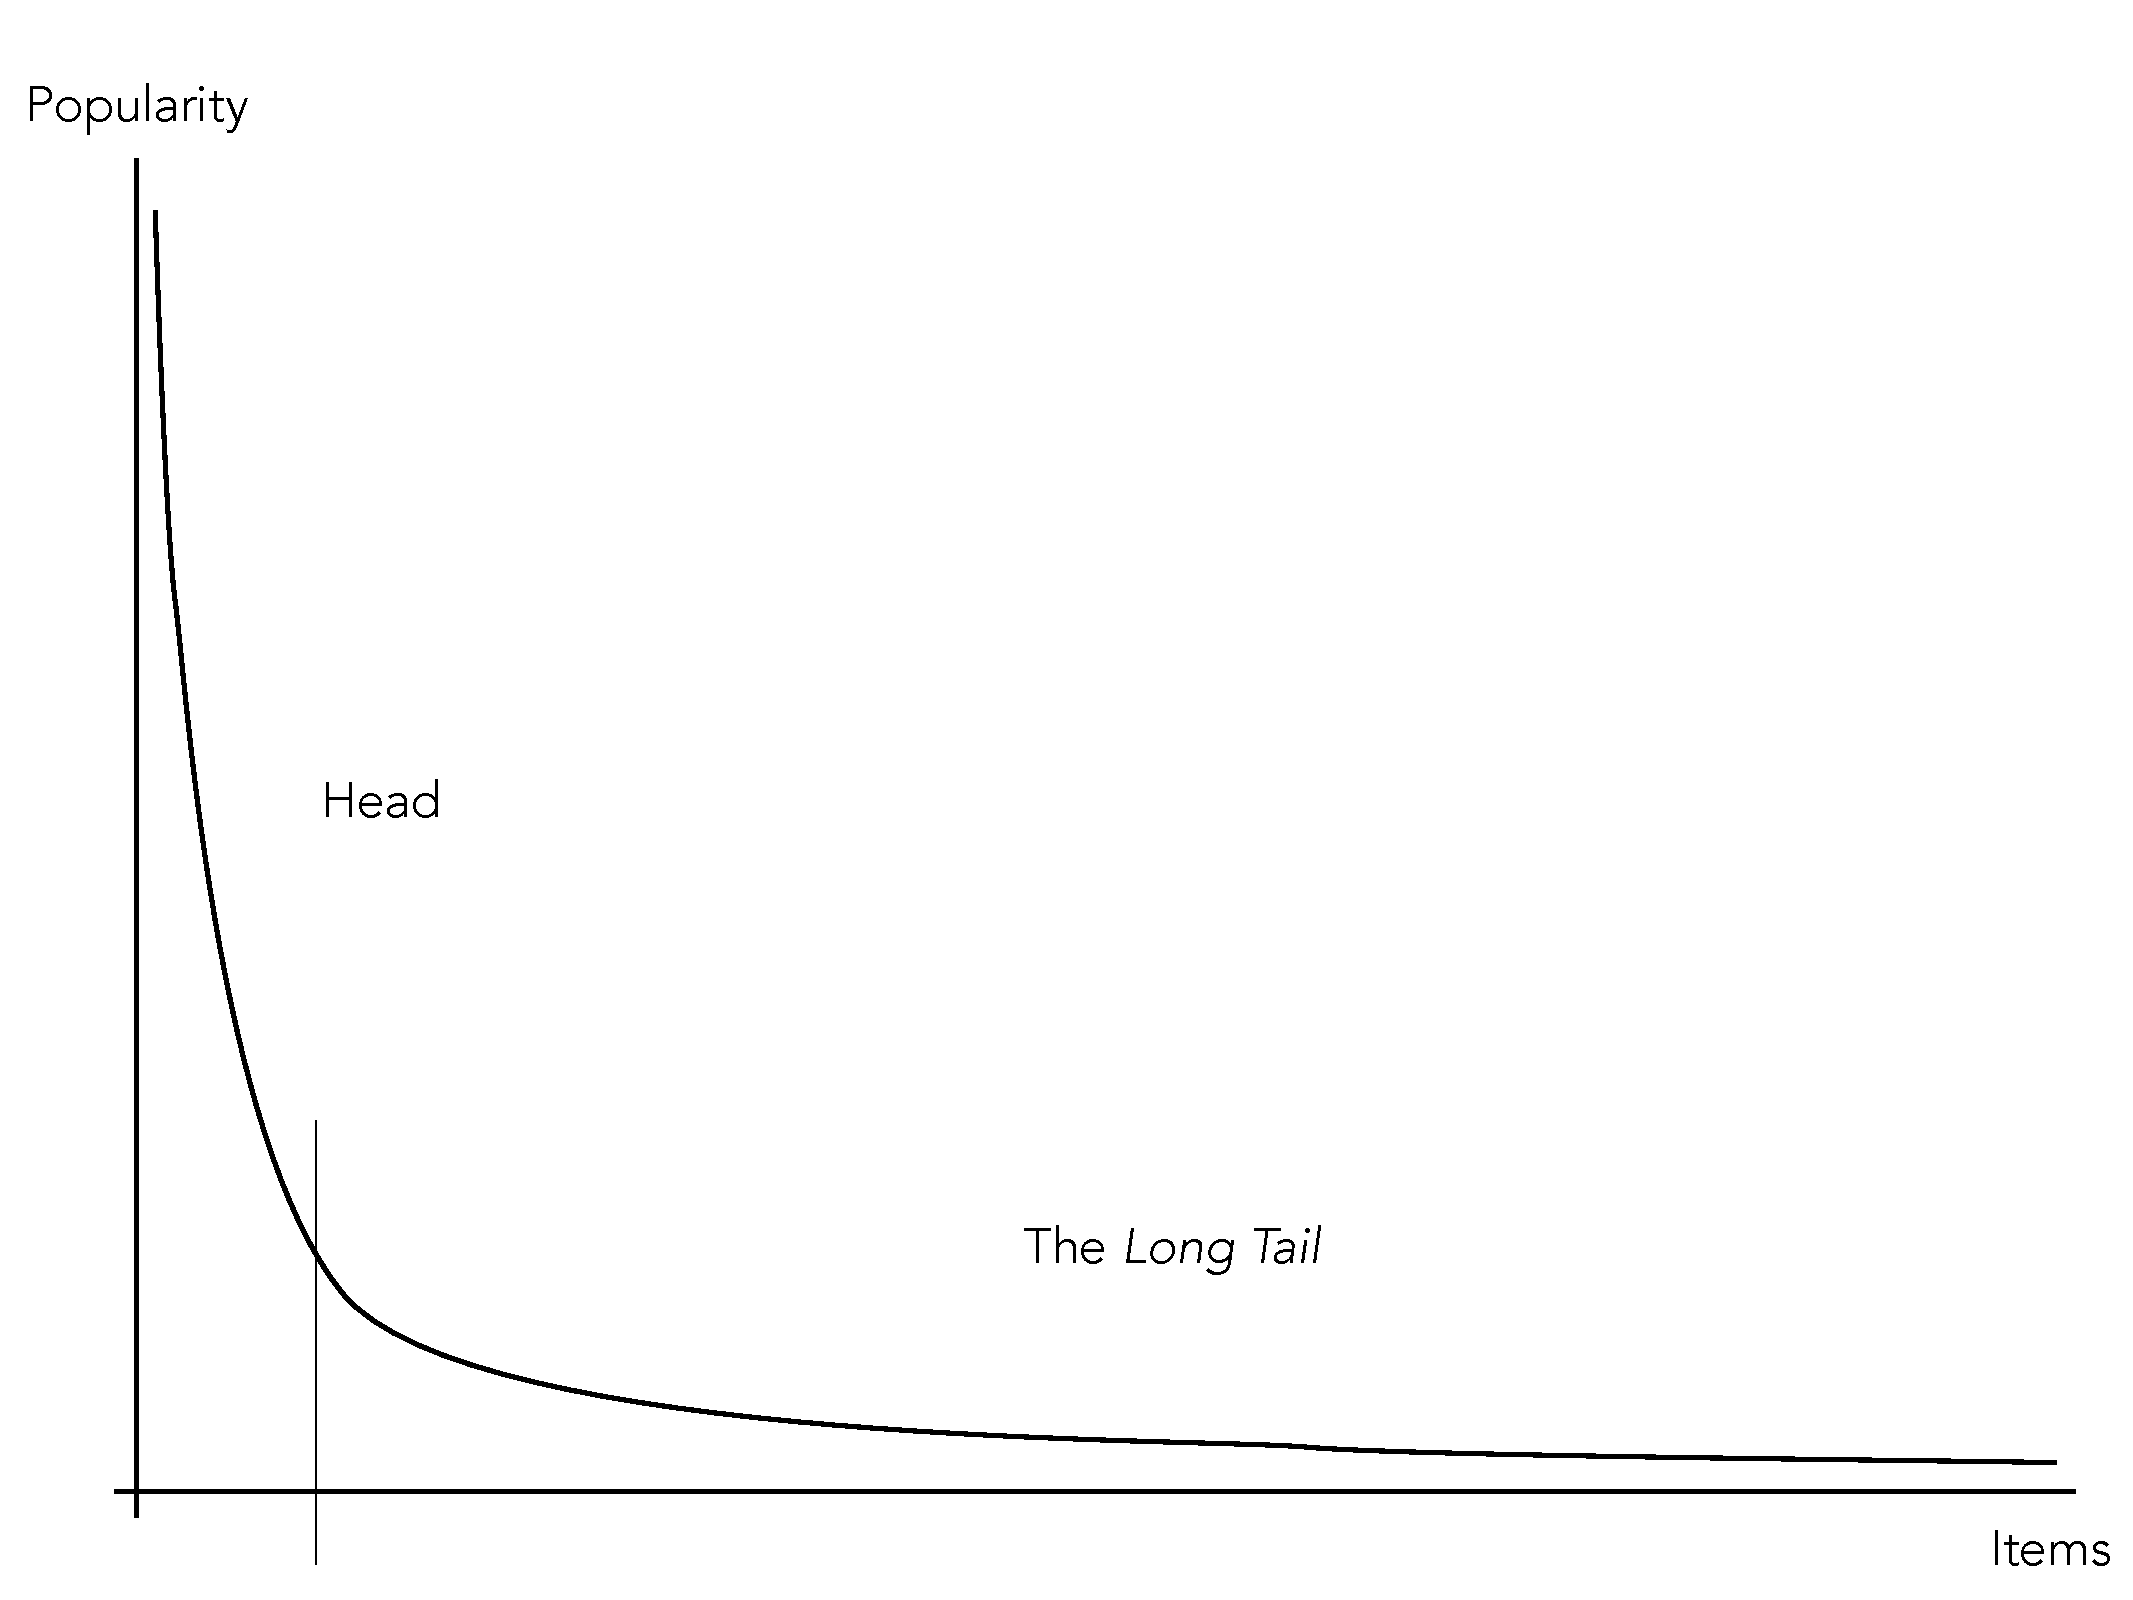
\includegraphics[width = 0.75\textwidth]{long_tail.pdf}
\caption[Ranking of popularity of a set of items exhibiting a long tail distribution]{Ranking of popularity of a set of items exhibiting a long tail distribution. The number of interactions with the most popular items in the head zone is similar to the number of interactions with the less popular items in the long tail.}
\label{fig:long_tail}
\end{figure}

% Novelty, relevance and the long tail
\textcite{celma10music} and  \textcite{celma11tutorial} suggested that among the many items in the long tail, modern recommendation systems should find and propose only novel and relevant items, otherwise users might find the recommended items non-interesting,  obvious, or simply driven by popularity. 
However, \textcite{bogt11moved} found that novelty is a characteristic that only some users want, typically those considered highly involved in music. 

It is reasonable to think that suggestions generated by a recommendation system should consider features such as novelty and relevance. But it also makes sense to follow \citeauthor{bogt11moved}'s finding and hypothesise that 
automated means of being exposed to less popular items are needed, but people are different and do not necessarily want to be exposed only to new items all the time. They may have different proclivity  for novelty, relevance, or other features. 

Incorporating profiling features within a customizable recommendation engine may help to create suggestions tailored to specific characteristics of listeners, such as how much they want to explore the long tail of items, or how similar is the music they want to listen to what everyone else is listening to. However, this is not straightforward when it comes to traditional approaches for recommendation.
The next section describes the main approaches for making recommendations. These approaches are based on characteristics of the items, of the users, or a combination of both.








\section{Recommendation approaches}\label{sec:4-recommendation-approaches}
Recommendation systems are information filtering agents designed to diminish information overload \autocite{good99combining}. They  operate under the premise of predicting which items a user will find worthwhile among a large set of items. 

The design and implementation of automated recommender systems generally falls into two different categories based on how recommendation are made:
\emph{content-based} (CB) approaches and \emph{collaborative filtering}-based (CF) recommendation. 
A third method, \emph{hybrid} recommendation,  is based on a combination of the two previous approaches \autocite{balabanovic97fab, adomavicius05toward}. 

CB approaches examine properties and features of the items to calculate their similarities, creating recommendations based on the degree of similarity between these features. 
\textcite{lang95newsweeder}, \textcite{pazzani96syskill}, and \textcite{chen98webmate} developed early recommender systems for the filtering of web pages and online news based on word frequencies and topics within the documents.

Instead of focusing on characteristics of the items, CF methods focus on behavioural relationships between users and items. These systems compute correlations or similarities between the interactions of users and items, and predict what items users may like based on those values. 
The earliest implementations of CF-based systems were put into effect for filtering out emails \autocite{goldberg92using}, online news and articles \autocite{resnick94grouplens}, and for the recommendation of music artists and albums \autocite{shardanand95social}.

Finally, hybrid approaches combine CB and CF in order to improve the overall performance of the  system \autocite{burke02hybrid}. 
For example, \textcite{balabanovic97fab} developed an early hybrid recommender based on word frequency as well as ratings given by users, that estimated the topics of webpages to recommend new webpages. 
In another example of the hybrid approach, \textcite{basu98recommendation} used editorial information about movies, such as metadata of the films and user-submitted tags, as well as a user's ratings on the movies, to improve the performance of a movie recommendation system.

The criteria, rationale, and an implementation overview of CB and CF-based recommenders are detailed in Sections \ref{sub:content} and \ref{sub:collaborative}, respectively. The techniques used for hybrid recommendation are based on combinations of CB and CF methods, hence are covered in those subsections. 
The specific ways in which CF approaches are implemented are detailed in Section \ref{sub:neighbourhood} for neighbourhood-based approaches, and in Section \ref{sub:model} for model-based approaches. Matrix Factorization, the most extensively used technique for CF is detailed in Section \ref{sub:matrix}.

% In this context, people might not be aware of the characteristics or the existence of the less popular items, and so being able to access them is highly improbable. 

% A comment on how collaborative filtering does not necessarily help to explore the long tail would be needed. Content-based methods seem to be better in this regards or, at least, agnostics to popularity.

% %%%%%%%%%%%%%%%%%%%%%%%%%%%%%%%%%%%%%%%%%%%%%%%%
% CONTENT-BASED RECOMMENDATION
% %%%%%%%%%%%%%%%%%%%%%%%%%%%%%%%%%%%%%%%%%%%%%%%%

\subsection{Content-based recommenders}\label{sub:content}
Content-based (CB) recommendation systems are based on information describing some inner characteristics of the set of items in their database \autocite{basu98recommendation}. 
By means of finding regularities among items' attributes, and using a sample of the user's preferences on these characteristics, CB information filtering systems estimate which items users may like, and suggest a subset of them to the user. 


% The process of characterizing an item can be automatized, by the automatically extracting features that describe some aspect of it, or manual, by having a set of domain experts annotating it~\textcite{su09survey}. Thus, finding good recommendation candidates is basically a procedure of finding similar items according to their distance in a chosen feature space. A similarity function is usually implemented for measuring the distance between items. Common distance metrics to compare feature vectors similarity are: \emph{Euclidian}, \emph{Manhattan}, \emph{Chebychev}, \emph{cosine distance}, and \emph{Mahalanobis} distances. Mathematical formulations for these distances can be find in section \ref{subsection:similarity_measures}. As CB recommendation systems do not rely on user ratings, these systems focus on objective distances, on the contrary that CF systems, which depend on users' subjective ratings \shortcite{celma10music}.


Many of the earliest information filtering systems used the CB approach for making recommendations. For example, \textcite{fischer91information} and \textcite{sheth94learning} created filtering systems for recommending online news based on the estimated topic of streams of articles. A similar approach was taken by \textcite{pazzani96syskill} for filtering websites. 
Recent commercial recommendation systems also rely on content for suggesting items. For example, the music streaming service Pandora\footnote{The Pandora Radio music streaming service is available at  \url{http://www.pandora.com}} automatically creates  playlists of songs by computing which songs in their database are similar to a given song provided by the user.


Instead of analysing the behavioural characteristics of users, or the interaction between users and items, CB recommendation systems rely primarily on describing items in the system by using a set of predefined features. This allow them to build a profile for each item based on attributes of its content. 
The process of characterizing the items is performed automatically by means of using automatic feature extraction, or manually by having a set of domain experts annotate the characteristics of the set of items. 
However, as the characteristics of items are domain-specific, it is not possible to generalise the set of features to extract. 
% For example, sets of common features that might be used to profile items in different domains could be:
For example, the following are sets of common features that may be used to profile items in different domains:


\begin{itemize}
\item For movies, users may want to pay attention to editorial metadata such as director, main actors, genre, studio, and year of production. 
\item For books, people can consider other books by the same writer,  books of the same genre, or other publications by the same publisher. Also, they may pay attention to the book summary or main topics. 
\item For music, people may pay attention to other pieces by performers, composers, or  writers they like. Other characteristics that people may pay attention are genre, instrumentation, tempo, or decade of production or release. Musically well informed listeners may also search for producers or labels.
\end{itemize}

Making recommendations by using a CB approach is achieved by finding those items that share similar characteristics with a given item.
Similarity of items can be decomposed in two main processes. The first process examines and determines the domain-specific features that describe the items in a dataset. The second process estimates the similarity between items in a set by measuring their distance in the feature space according to a given metric.
The next two subsections review the characteristics of audio features for describing musical signals, and some of metrics to measure similarity in  feature spaces.



\subsubsection{Audio features for describing musical signals}
There is not a single, unique way to describe a piece of music. Depending on the characteristics of the song that we want to pay attention to, different aspects of the audio can be relevant. For example, two songs can share similar harmonic content, but can differ greatly in tempo, rhythmic characteristics, or melody.
By applying digital signal processing techniques to the audio signal of music tracks, we can perform calculations on its physical quantities as they evolve over time, and use that information to characterise some intrinsic attributes of the songs.

Features extracted from audio signals are known as signal-based, audio-based, or con\-tent-based \autocite{schedl12useraware}. Depending on the level of abstraction about the musical content, these features can be low-level, mid-level, or high-level representations of the audio information. 
Low-level features are calculated straightforwardly by computing systems because they are quantified directly from the audio signal. However, most low-level features do not convey a direct musical meaning to listeners, or are only loosely correlated \autocite{gouyon08content}. Mid- and high-level features typically require the aggregation of low-level data into higher-level representations, but in contrast to low-level features, these characterisations often approximate perceived musical attributes such as the genre, mood, or instrumentation of a song. 
However, in order to capture those musical attributes, complex models may be necessary in order to estimate these higher-level descriptions of the audio signal \autocite{van13deep}.



Audio feature extraction was defined by \textcite{tzanetakis02musical} as the process of computing a compact numerical representation that is used to characterise a segment of audio.
Numerical values for the audio features are calculated using digital signal processing techniques. In these techniques, an audio signal is digitised and converted into a standard audio file format with a fixed sample rate. Then, the signal is divided into frames, short segments of audio, where it is assumed that the feature values will remain stationary. 
A window function is applied to each of these frames in order to minimise the discontinuities at the beginning and end of each frame. Adjacent windows usually overlap in order to obtain smoother analyses. 
Numerical values for all wanted audio features are computed for each windowed audio segment. 
Finally, an aggregation of these time-varying values is performed to create a summary for each feature.
By using the derivatives instead of the instantaneous values it is also possible to account for the temporal evolution, or degree of change, of the feature values. 

The various representations of the audio signal are used to extract features that allow the attributes of the signal to be characterised from different perspectives. 
For example, the temporal representation of the audio frames is used to extract so-called temporal features, such as amplitude and energy of samples within each frame, zero-crossing rate, temporal centroid, auto-correlation coefficients, and pitch features among others. 
On the other hand, the spectral representation of the audio signal is used to compute so-called spectral features, such as the spectrum energy, and mean, spread, centroid, flatness, kurtosis, skewness, spectral slope, and roll-off of the spectrum frequency distribution. 
Cepstral features, such as Mel-Frequency cepstrum coefficients (MFCC), are low-level characterisations of the audio signal derived from a transformed version of the spectrum that capture some timbral aspects of music \autocite{gouyon08content}.
Rhythmic content features, such as the beat histogram of an audio signal, are extracted from a combination of the previous representations with the goal of representing the rhythmic structure of music \autocite{tzanetakis02musical}. 

Musical features of higher level can be computed by means of the aggregation of features of lower level extracted from the audio signal. For example, note onset detection and intra-note segmentation are features that describe the starting point, attack, sustain, and release of musical notes. These points can be calculated from the temporal variations of single or multiple low-level features, such as changes in the audio signal's energy and pitch \autocite{gouyon08content}.
Describing high-level musical concepts such as timbre, harmony, melody, rhythm, genre, or instrumentation, requires the design, implementation, and evaluation of even more complex models. 


The Music Information Retrieval Evaluation eXchange (MIREX)\footnote{The Music Information Retrieval Evaluation eXchange (MIREX) webpage is available at \url{http://www.music-ir.org/mirex/wiki/MIREX_HOME}} is an annual evaluation campaign where algorithms relevant to music information retrieval tasks are compared by using same datasets and evaluation procedures \autocite{downie08music}. 
The tasks of the competition are defined on a yearly basis and the outcome of the contest is a ranking of the submissions per task. In the 2016 competition, those that received the largest amount of submissions were: onset detection, singing voice separation, audio melody extraction, audio chord estimation, audio beat tracking, and structure segmentation \autocite{downie16mirex}. The larger amount of submissions in these tasks can be a signal as to the current research interests of the music information retrieval community. 
The MIREX evaluation campaign is a key point of reference when looking for the current state-of-the-art research in musical features extraction. 
The systems and algorithms presented in MIREX can be used by researchers and developers to implement sophisticated music recommendation systems and models based on audio feature extraction and aggregation.

% \begin{description}
% 	\item [Audio melody extraction ] aims to identify the melodic pitch perceived from polyphonic musical audio. Pitch is expressed as the fundamental frequency of the main melodic voice, reported for each frame on an evenly space time grid. The actual pitch detection task implies deciding the most likely melody pitch for each frame. 
% 	Fundamental frequency $f_0$ is the main low-level feature to describe aspects of melody. Different cases of pitch detection are \emph{fundamental frequency estimation of monophonic sounds}, \emph{multi-pitch estimation}, and \emph{predominant pitch estimation}. In a rudimentary explanation, the calculation of a single $f_0$ in monophonic sounds is performed by estimating the fundamental frequency based on temporal or spectral aspects of each analysis frame, and smoothing the resultant contour. Typical time-domain algorithms use low-level zero-crossing rate or time-domain autocorrelation function. Common frequency-domain algorithms are based on cepstral fundamental frequency detection or spectrum autocorrelation methods. Multi-pitch and predominant pitch estimation are more complex cases. While algorithms for the former benefit from the perceptual fusion of auditory streams, algorithms for the later assume that predominant instruments define the melody.For melodic extraction from a musical background, different techniques aim to identify notes that correspond to the melody. While some of them try to detect note groupings based on heuristics passed to computational models, others make assumptions on the type of music analyzed~\autocite{gomez03melody}. 
% 	The approach by \textcite{salamon11melody}, currently the most accurate algorithm in the MIREX context, uses a four-step approach of sinusoid extraction, salience function computation, pitch contour creation, and melody selection. The authors used two different signal processing techniques for sinusoid extraction based on the STFT, and multi-resolution Fast Fourier Transform, achieving similar results.

% 	\item [Audio tempo extraction ] techniques aim to extract the tempo from musical audio. Typical tempo extraction is achieved on two stages. First, a representation of temporal dynamics is obtained from the audio by taking the derivative of the signal energy in a number of frequency bands. Second, periodic regularities in the signal of the first stage are tabulated through the use of resonator filter banks, multi-agent methods, or probabilistic models. The tabulation of the periodicities generate a single value or a list of candidate values that represent the tempo of a piece of music ~\autocite{mckinney04extracting}.
% 	However, tempo can be distinguished between ``annotated'', the official annotated tempo of a piece, and ``perceived'', the one that people follow in probably different metrical levels. The MIREX audio tempo extraction task goal aims to extract the perceived tempo. The current winner algorithm by \textcite{gkiokas11ilsp} uses a percussive/harmonic separation algorithm of the audio signal to extract filterbank energies and chroma vectors. Periodicity analysis is performed in these feature vectors, and a target tempo is estimated from the resulting periodicity vector.

% 	\item [Audio genre classification ] task goal is to automatically classify a polyphonic musical audio signal into a high-level genre. As pointed out by \textcite{mckay06musical}, genre classification is particularly difficult because it assumes culturally predetermined classes in which even humans agree only to a limited extent. As such, a piece of music can belong to several genres to varying degrees, the understanding of what a music genre is can evolve over time, and new genres are introduced regularly. Notwithstanding, genre classification has had a large amount of research. Approaches for music genre classification have been typically based on training a model with feature vectors extracted from musical audio signals from a ground truth dataset, and then testing the model in new data. As the basis of any automatic audio analysis system that tries to characterize aspects of the audio signal is the extraction of feature vectors, and because genre is a very complex topic, many features, of diverse domains, have been tested. \emph{Timbral texture features}, such as the spectral and cepstral features described above have been used to represent the timbral texture of a music audio signal; \emph{rhythmic content features}, such as the beat histogram, have also been used to characterize rhythmic aspects of genre such as the running estimate of the main beat and its strength, the regularity of the rhythm, and the relation of the beat to sub-beats. Also, \emph{pitch content features} such as the most dominant pitch class of the song, the octave range of the dominant pitch, the main tonal interval relation, and pitch histogram, have been used to characterize the pitch content and relations of musical pieces. ~\textcite{tzanetakis02musical} report that timbral texture features perform better than rhythmic and pitch features, but the integration of all three set of features together achieves even better performance, meaning that each set provides some unique information about musical genre and musical content in general.
% \end{description}


Features to describe the musical content from audio signals have been used since early music recommendation systems. For example, \textcite{welsh00querying} developed a system aimed to help people navigate similar-sounding songs. Their approach was based on the automatic extraction of more than 1,000 audio features per track that described temporal, spectral, rhythmic, and higher-level characteristics such as genre of tracks in their system's data\-base.
% This way of estimating the closest items is common in music recommendation based on acoustic features. 
A user then provided a seed song, the set of features was computed for the track if they were not already computed, and the system retrieved and suggested the nearest neighbour tracks in the feature space.
\citeauthor{welsh00querying}, however, did not provide any measure of the effectiveness of their system due to the ``subjective nature of similarity.'' 

Similarly, \textcite{tzanetakis01automatic} developed a set of features for representing texture and instrumentation of audio signals, and a set of algorithms for automatic genre classification. Their features aimed to represent the ``musical surface'' of audio: timbre, texture, instrumentation, and rhythm.
By using dimensionality reduction techniques the authors mapped songs into a lower dimensional space, aiming to have songs of the same genre close to one another in the resultant feature space. 
\citeauthor{tzanetakis01automatic} also developed a graphical user interface to browse and interact with the set of songs, songs collections, or audio signals in general.  The interface aimed to allow users to navigate these sound objects, which were clustered by similarity in the space. They did not provide any evaluation of their system or interfaces.

There are some conceptual caveats in estimating similarity using a CB approach. First, \textcite{slaney08learning} pointed out that the very concept of similarity in music is an ``ill-posed problem:'' it is likely that two people may disagree about the degree of similarity between two songs, and so the ground-truth information extracted from their direct observation is not conclusive. \textcite{van13deep} elaborated on this idea, and stated that there is also a semantic gap between low-level features describing a set of musical items and what users recognise as something perceptually relevant. They noted that most metrics for measuring perceptual similarity are defined based on prior, expert knowledge in the domain of the items to be recommended, but they are not optimal for the task of music recommendation because of the semantic gap.
As a result, \citeauthor{van13deep} investigated an approach that did not use a set of predefined features to estimate similarity, but instead a model learnt a set of latent factors from the audio signal and used these to estimate song and artist similarity.




Despite the previously mentioned caveats, automatic approaches for audio signal classification similar to the aforementioned have been implemented in commercial audio recognition and music recommendation systems such as Mufin.\footnote{The audio identification and music recommendation company Mufin is available at \url{http://www.mufin.com}} 
Alternatively, manually driven descriptions of tracks have been used in the recommendation systems of commercial music streaming services such as Pandora.
Pandora's documentation states that ``music analysts with a four-year degree in music theory, composition or performance'' manually annotate up to 450 features for characterizing each song using ``precisely defined terminology,'' as part of the so-called Music Genome Project,\footnote{An overview of the Music Genome Project is available at \url{http://www.pandora.com/about/mgp}} patented by \textcite{glaser06consumer}. 
However, beyond the general information in the patent itself there is no publicly available description about the features themselves, the feature extraction process, or the metrics used by Pandora and the Music Genome Project \autocite{turnbull08dissertation}. 

% scalability and trust
Automated feature extraction has the greatest impact on the scalability of a recommendation system because it allows for faster, inexpensive, and more consistent annotations than manually characterised items \autocite{brandenburg09music}. 
On the contrary, annotations made by human experts allow for the extraction of more reliable and higher-level features \autocite{tingle10exploring}. 
As a result, while companies that rely on automatic approaches for feature extraction are able to annotate and manage huge datasets of items, institutions and services that use annotations made by experts usually have  smaller but more detailed datasets. For example, Pandora has a song corpus one order of magnitude smaller than other music streaming services \autocite{sydell14pandora}, but according to marketing research by \textcite{infinitedial15}, it has been the music streaming service leader in the United States for several years.

% Also, using domain experts might imply that higher-level features could be extracted, but with probably less uniformity in the appreciation, or measurement, of features.

% For example, in the context of content-based music recommendation, the similarity of a set of songs can be computed based on audio feature vectors extracted from low-level acoustic features such as energy or mel-frequency cepstral coefficients (MFCCs), and also from high-level features describing the track, such as its genre or instrumentation~\autocite{bogdanov09low}. 
% Then, given a user-provided \emph{seed} song, recommendations are generated by estimating what are the songs that are closest to the user-given song in the feature space~\autocite{casey08content}.

% Recommendations are then generated by asking the user to provide a \emph{seed} song, computing the features of this seed track (if the features are not already calculated), and finding those items which are closer to the user-provided song in the feature space~\autocite{casey08content}. 

% If we think that the set of feature values place each one of the items in one point in a multi-dimensional space. 


Once the set of domain-specific features that characterise a set of musical items has been designed and implemented, the remaining question is how to calculate the distance between these items' projections into the multi-dimensional feature space. The next subsection provides a review of similarity metrics that allow us to estimate this distance.
Mathematical formalizations, implementation details, and examples of use about some of these similarity measures are given in Section \ref{sub:neighbourhood}.

\subsubsection{Similarity measures}
Similarity functions aim to estimate the likeness of items in a given multi-dimensional space, yielding numerical, real-valued metrics based on different approaches. The chosen method can greatly impact the resulting similarity measure, and so it is important to consider the characteristics of the data as well as the characteristics of the features describing the data when choosing a specific approach.

The most straightforward methods estimate the similarity of items by calculating pair-wise distances along all dimensions of the feature space. 
Euclidean distance simply measures the straight distance between two items in the multi-dimensional space to yield a similarity metric.
Manhattan distance also computes the distance between two points in  space, but it aggregates the distances along the grid lines of the axes to estimate the similarity of items. As a result of this rectilinear approach, it is also known as taxicab distance.
These two distance-based metrics assume that the features have similar scale, and so they have similar perceptual relevance; and also that the features are relatively independent and so the distance can be summed up along the axes.

Instead of using distances between points to calculate their similarity, the cosine similarity metric calculates the cosine of the angle that two feature vectors form in space to estimate their similarity. As a result, similar items will have similarity values close to $0$, and dissimilar ones will have values close to $\pm 1$, depending upon the angle between them.

The Jaccard distance estimates the similarity, or difference, of items as a set problem. This metric functions by computing a numerical value using the intersection and union of sets of items. Therefore, it is well-tailored for cases with categorical variables, or for cases in which the items are described by a subset of all features.

Finally, Mahalanobis distance calculates the similarity between points by computing the distance between a point and the centre of mass of a given set of points. This estimation of distance is estimated in terms of the number of standard deviations between them. As a result, it yields a value predicting if the point belongs or not to cluster of points which is unit-less and scale-invariant.




As described in previous sections, CB recommenders operate by first defining a set of features to describe intrinsic characteristics of items, and then defining a metric to measure the similarity of these items according to the chosen features.
As a result, these systems consider items that are in the head of the popularity ranking of the probability distribution curve in the same way as items at the very end of the long tail. 
In this sense, recommendations made by CB systems are not biased by pre-existing preferences of users, or their perception about items, as well as being less mediated by marketing campaigns or media exposure of a chosen group of items. 
This characteristic of CB recommendation allows people to explore a whole dataset of available items much more deeply, because the recommendation process is not biased by previous preferences.
However, it is also possible to make many non-interesting or non-relevant recommendations by means of measuring the similarity of tracks based on a set of low-level or high-level features. Recommending music is more than just paying attention to acoustic properties of the audio signal. 
A series of methods relying on a different approach were developed in order to find more relevant items. We now proceed to describe CF recommendation, an approach to recommendation that is agnostic to the actual content or metadata of items. 


% ~\textcite{slaney08learning} pointed out that the very concept of similarity in music is an ``ill-posed problem'': it is likely that two people may disagree about the degree of similarity between two songs.
% ~\textcite{van13deep} stated that a semantic gap exists between the low-level features describing a set of items and what the users recognize as something perceptually relevant. They noted that most metrics for measuring perceptual similarity are defined based on prior, expert knowledge in the domain of the items to be recommended, but they are not optimal for the task of music recommendation because of the semantic gap.
% As a result, \citeauthor{van13deep} investigated the use of deep convolutional neural networks to predict latent factors from music audio, an approach that does not actually use a set of predefined features.





% comprehensive review on CF  {ekstrand11collaborative}



\subsection{Collaborative filtering recommendation}\label{sub:collaborative}
% NETFLIX Prize
A different approach to create recommendations is collaborative filtering (CF), term coined by \textcite{goldberg92using}. The fundamental assumption of this recommendation method is based on the idea that if two individuals assign similar ratings to a set of items---or behave similarly with them---those people share similar tastes and therefore may rate or act on other items similarly. 
Therefore, CF recommendations base their approach on usage by aggregating the preferences on items of a large amount of users and  recognizing the commonalities or similarities between users on the basis of their choices. Finally, CF recommendation approaches generate suggestions based on inter-user comparison.
Since these systems do not need especially hand-crafted features to describe the set of items, they have the advantage of being agnostic to the domain of the items.
% These systems just need information  expressing their preference on a set of items.

\textcite{slaney11web} pointed out that CF outperform CB systems at the large scale of the Internet in many item domains because they take into account people's perceived similarity of items. Previously, \textcite{slaney07similarity} designed an experiment in which a large number of users had to judged the similarity between a set of playlists. 
The playlists were generated by: (i) CB similarity using state-of-the-art acoustic feature extraction algorithms, (ii) explicit ratings of a large amount of listeners on songs, and (iii) a random playlist generator that was used as a baseline.
The authors found that listeners preferred the playlists based on usage much more than the ones based on content.
Consequently, CF is currently the dominant and most successful framework for recommending media items and items in general \autocite{shi14collaborative}, driving the recommendation frameworks of major media delivery companies such as Amazon \autocite{linden03amazon}, Netflix \autocite{gomez15netflix}, and Spotify \autocite{johnson14logistic}.


However, CF systems suffer from some issues. For example, since these systems rely on usage data, they can only generate recommendations for those users and items for which the system has enough information. This problematic issue was described by \textcite{maltz95pointing} as the \textit{cold start} problem of CF systems. New users usually start with an empty profile, and so it is not possible to find other users with a similar set of preferences to generate good recommendations. Similarly, new items that have not been experienced by anyone will be unlikely to be recommended by the system. Therefore, during the cold start period a recommendation system will not be able to effectively filter and suggest items to users. 

The cold start effect is particularly important in the domain of media and music. \textcite{celma10music} pointed out that the consumption of music items follow a power-law distribution, therefore the largest proportion of the least popular items is experienced by listeners much less than the smallest proportion of the more popular music items. As a result, generating recommendations for the less-preferred music entities has a much smaller probability. In other words, the more popular items will be suggested more frequently by CF recommendation systems than the less popular items, and this phenomenon will be reinforced over and over, as a feedback loop.


% The implementation of CF recommender systems, mathematical formalizations for these implementations, and synthetic general examples and music-domain examples are provided in the next section.

% \subsection{Approaches for collaborative filtering recommendation}

CF-based recommendation can be implemented by means of different conceptual approaches. 
While all these methods aim to find a set of like-minded users given a seed user, or a set of similarly consumed items according to a seed item, the estimation of similarity between the users or items is achieved by different means.
The primary methods used to compute this similitude are: (i) computing the correlation of users' previous preferences on items, and (ii) learning a model based on these preferences, model which is used afterwards to estimate future preferences. These two strategies are commonly denominated neighbourhood or memory-based,  and model-based approaches. These processes are detailed in the next sections.

% Also, $\lambda$ is used as the letter for write the regularization parameter used to control the magnitudes of estimated values in a model, thus helping to control the overfitting the sparse data of the rating matrix.

% A couple of baseline values are also usually defined to account for biases in the data. Thus, $\mu$ is the global bias term, i.e., the overall average rating. The deviations from the average of user $u$ and item $i$ are written as $b_{u}$ and $b_{i}$, respectively, and can be interpreted as the biases of each user and item. Hence, the baseline value for an unknown rating $r_{ui}$ consists in global bias, and the user and item biases:

% % Formula from koren08factorization
% \begin{center}
% \label{eq:basline_value}
% $b_{iu} = \mu + b_u + b_i $
% \end{center}


\subsection{Neighbourhood approaches}\label{sub:neighbourhood}
Neighbourhood-based recommendation is based on the idea that people rely on like-minded people or sources to evaluate the recommendation value of an item. This concept is colloquially known as recommendation by word-of-mouth \autocite{ricci15recommender}. People recognise as good recommendations those suggestions made by others who they believe to have similar interests.
Therefore, neighbourhood-based recommendation systems aim to find a subset of entities---users or, alternatively, items---with similar behaviour within the pool of entities of the dataset.
The interactions of all users on items are stored in a database of events. These interactions are aggregated and mapped onto a two-dimensional space that allows to perform faster calculations.
The similarity between users or items is computed by comparing the rating patterns of users or items, which is then used to find the nearest neighbours. Hence, neighbourhood-based methods generate predictions on not-yet experienced user-items interactions based on past preferences \autocite{herlocker99algorithmic}.
% It is common in recommendation settings that users only interact with a very small portion of all available items, and so the matrix of interactions---known as the \emph{utility matrix}  or \emph{rating matrix}---is usually fairly sparse. This sparsity effect can be an issue since the number of preference values to be estimated is much larger than the number of known preferences. This is especially relevant for predicting preference values for the many items in the long tail . %~\autocite{goldberg01eigentaste}


\emph{User-based} neighbourhood systems try to predict the preference of a target user on an item, given the rating of similar users---those with similar rating patterns---on that item. 
In other words, the rating ${\hat{r}}_{ui}$ of user $u$ on item $i$ can be predicted given a set of $k$ like-minded similar users and all ratings that the $k$ users have given to the item $i$.\footnote{A note on notation. Throughout this chapter we use the same notation used by \textcite{koren08factorization}, where letters $u$ and $v$ represent users, and $i$ and $j$ are used to represent items. A rating indicating the preference of user $u$ on item $i$ is written as $r_{ui}$. If rating $r_{ui}$ is predicted, instead of actually rated, it is written as ${\hat{r}}_{ui}$.}
The interaction between user $u$ and item $i$ is notated as the item pair $(u,i)$, and all interaction pairs are stored in a set $\mathcal{K}$, hence $\mathcal{K} = \{(u,i)\ |\ r_{ui} \textrm{ is known} \}$. 
The estimated rating ${\hat{r}}_{ui}$ is computed as the average rating given to $i$ by the subset of neighbours, usually weighted by their degree of similarity with the user $u$, and considering any bias in their ratings.

% actual rating: 		$r_{ui}$
% estimated rating: 	${\hat{r}}_{ui}$


In contrast to user-based techniques, item-based neighbourhood recommendation systems try to predict the rating of users on items using previous ratings given by users to similar items (i.e., those items with similar rating patterns).
In this technique, a set of $k$ similar items is used to predict a rating ${\hat{r}}_{ui}$ of user $u$ on item $i$, given the ratings that $u$ has given to the $k$ items.
The estimated rating ${\hat{r}}_{ui}$ is computed as the weighted average of the ratings given by $u$ to the $k$ items. %The degree of similarity and bias are usually also considered.

As computing the similarity between users or items is a key component in neighbourhood approaches---all predictions are based on the similarity between entities in the system---the computation of a suitable similarity metric is a crucial component in building a neighbourhood-based recommendation system.
Similarity functions combine the set of ratings of users on items into a single value that represents the similarity between entities, users or items. 
This value can be also interpreted as the degree of influence or weight when calculating the predicted rating of one entity on another.

There are several different methods for estimating similarity, but  \textit{Pearson correlation}, \emph{Cosine Vector similarity}, and \emph{Jaccard similarity} are the ones more commonly used in recommendation systems \autocite{leskovec14mining, ricci15recommender}. We provide details about the computation of these three similarity metrics in the following subsections.


\subsubsection*{Cosine vector similarity}\label{subsubsection:cosine_vector}
Also known as \emph{Cosine distance}, this metric computes the similarity between two entities $i$ and $j$ by calculating the cosine of the angle that the two vectors $\vec{x}_i$ and $\vec{x}_j$ form \autocite{salton83introduction}. The smaller the angle the vectors form, the more similar the two entities are.   

For example, two different music tracks $i$ and $j$ can be characterised by a set of features representing some of their musical attributes. Numerical values for these features are stored in vectors $\vec{x}_i$ and $\vec{x}_j$. Each of these vectors can be visualised as a segment that connects the origin of the multi-dimensional feature space to a specific point in this space.
Cosine vector similarity calculates the angle these two vectors form. If the two items are similar, the angle their vectors form will be small. Cosine vector similarity is formalised as the dot product of the vectors divided by the product of their norms:
% Formula from ricci15recommendation, pp.53
% \begin{figure}[ht]
% \centering
% \includegraphics[width = 0.3\textwidth]{cosine_similarity_formula.png}
% \caption{Cosine similarity}
% \label{fig:cosine_similarity_formula}
% \end{figure}
% Formula from ricci15recommendation, pp.53
\begin{equation} 
\label{eq:cosine_vector_item_similarity}
\text{cos}(\vec{x}_i, \vec{x}_j) = 
\frac
{
% 	\vec{x}_i^\top \vec{x}_j 
    \vec{x}_i \Bigcdot \vec{x}_j 
}
{
	\|\vec{x}_i\| \|\vec{x}_j\|
} 
% \vspace{1em}
\end{equation}


In recommendation settings, Cosine vector distance is used to compute the similarity between users $u$ and $v$, given a set of items $\mathcal{I}_{uv}$ that has been rated in common by the users. 
% The Cosine vector distance metric uses the set of rating values to compute the similarity between the pair of users. 
Hence, Cosine vector-based similarity between users $u$ and $v$ is formally written as follows:
% Formula from ricci15recommendation, pp.53
\begin{equation}
% \vspace{1em}
\label{eq:cosine_vector_user_similarity}
sim_{CV}({u,v}) = 
\text{cos}(\vec{x}_u, \vec{x}_v) = 
\frac{
\displaystyle\sum_{i \in \mathcal{I}_{uv}}r_{ui} r_{vi}} 
{ 
\sqrt
{
\displaystyle\sum_{i \in \mathcal{I}_u}r^2_{ui} 
\displaystyle\sum_{j \in \mathcal{I}_v}r^2_{vj}}
} 
\vspace{1em}
\end{equation}
where $\mathcal{I}_{u}$ and $\mathcal{I}_{v}$ correspond to the items that users $u$ and $v$ have respectively rated, and $\mathcal{I}_{uv}$ corresponds to the set of all items that users $u$ and $v$ have rated in common.

Measuring the similarity between users $u$ and $v$ with Cosine vector distance has the drawback of not considering the variances of the ratings of each user. 
As a result, the estimated similarity between users that use different scales to rate items may be misleading, because their personal biases are not considered in the calculation.
In order to account for probable biases in ratings given by users, a different similarity metric is commonly used in recommendation settings. This metric is the Pearson correlation.

\subsubsection*{Pearson correlation}\label{subsubsection:pearson_correlation}
Pearson's correlation coefficient is used in recommendation settings to measure the similarity between users or items that incorporates the mean of the rating values as part of its computation. By incorporating this value, it normalises the values of the vectors to their arithmetic mean \autocite{resnick94grouplens}.
Thus, the Pearson correlation-based similarity between users $u$ and $v$, where $i \in \mathcal{I}_{uv}$ corresponds to all items that have been rated by both users, and $\bar{r}_u$ and $\bar{r}_v$ are average ratings of co-rated items by users $u$ and $v$, is formalised as follows:
% % Formula from ricci15recommendation, pp.54
\begin{equation}
% \vspace{1em}
\label{eq:pearson_correlation_user_similarity}
sim_{PC}({u,v}) = 
% \frac{
% cov(u,v)
% }
% {
% \sigma_{u} \sigma_{v}
% } 
% = 
\frac{
\displaystyle\sum_{i \in I_{uv}}(r_{ui} - \bar{r}_u)(r_{vi} - \bar{r}_v)
}{
\sqrt
{
\displaystyle\sum_{i \in I_{uv}}{(r_{ui} - \bar{r}_u)}^2 
\displaystyle\sum_{i \in I_{uv}}{(r_{vi} - \bar{r}_v)}^2
}
}
\vspace{1em}
\end{equation}



Pearson correlation is similar to Cosine similarity. However, instead of having a fix origin, the origin is translated to the arithmetic mean of the vectors \autocite{egghe09relation}. Consequently, this translation allows to obtain correlation-based similarity values within the range $\pm$1, while Cosine vector-based similarity varies only from zero to one.

Although the two aforementioned are the most used similarity metrics in the context of recommender systems \autocite{leskovec14mining, ricci15recommender}, there is also another metric known as the Jaccard similarity index, which is based on the idea of set similarity.



\subsubsection*{Jaccard similarity}\label{subsubsection:jaccard_similarity}
Jaccard similarity is a metric based on the presence or absence of a set of attributes instead of the actual value of those attributes. Jaccard similarity measures how close two sets are, resulting in higher values when the sets are similar to each other. 
In recommendation settings, this metric can be interpreted as a measure of the similarity of the set of items experienced by users, but not considering the actual preference values on those items. Jaccard similarity is formalised as follows:
% Formula from ricci15recommendation, pp.54
\begin{equation}
\label{eq:jaccard_similarity}
sim_{JS}({A,B}) =
\frac{
|A\cap B|
}{
|A\cup B|
}
% \vspace{1em}
\end{equation}
where $A$ and $B$ can be any set of elements, such as the sets of rated items by users or the presence or absence of categorical item features. 




% %%%%%%%%%%%%%%%%%%%%%%%%%%%%%%%%%%%%%%%%%%%%%%%%
% SYNTHETIC RATING MATRIX
% %%%%%%%%%%%%%%%%%%%%%%%%%%%%%%%%%%%%%%%%%%%%%%%%


\subsubsection*{Synthetic example of similarity measures}
In order to exemplify similarities and differences between the three aforementioned similarity metrics, we now present an example of their behaviour in a small synthetic dataset.
In this dataset a set of users $U=\{u_{1}, u_{2}, \ldots ,u_{5}\}$ expressed their opinions about a set of items $I =\{i_{1},i_{2}, \ldots ,i_{10}\}$ in the form of preference ratings in a 1-to-5 scale. 


% \vspace{1em}
Table \ref{table:rating_matrix_1} shows the synthetic utility matrix with the rating values for all interactions between users and items.
Most users have expressed their preference for $i_{1}$ and $i_{5}$, however just a few have expressed preference for $i_{2}$, $i_{3}$, $i_{3}$, $i_{6}$, or $i_{8}$. 
In fact, all users of this synthetic dataset have expressed preference only for some of the items. For example, users $u_{2}$, $u_{3}$, $u_{4}$, and $u_{5}$ have expressed preference for just half of the items. 

The sparsity of the expressed preferences in Table \ref{table:rating_matrix_1} is common in rating matrices, but actual rating matrices have a much larger sparsity than the one shown in this synthetic example. 

\begin{table}[!ht]
\vspace{1em}
\centering
\caption[Synthetic example of rating matrix]{Synthetic example of rating matrix. A set of users $U$ have expressed their preferences on a set of items $I$. Only a portion of the items have been rated.}\label{table:rating_matrix_1}
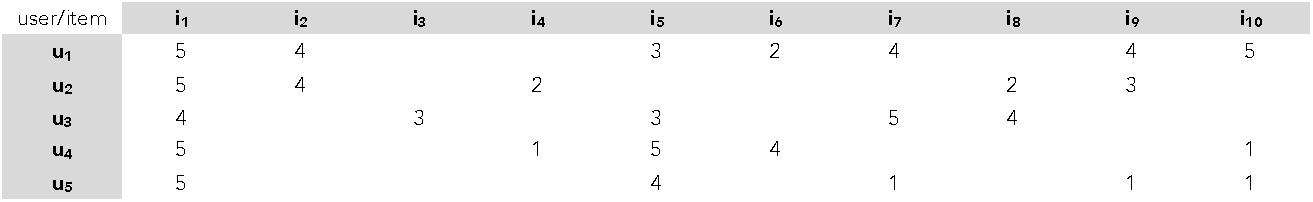
\includegraphics[width = 1.0\textwidth]{rating_matrix_1.pdf}
\end{table}



We now assess user similarity with the three previously described metrics. The three sets of similarity values are presented in Table \ref{table:similarity_metrics_comparison}. 
\begin{table}[ht!]
\caption[Assessment of user similarity with different measures of simmilarity]{Assessment of user similarity in synthetic dataset using (a) Cosine vector, (b) Pearson correlation, and (c) Jaccard similarity metrics. Most similar pairs for each metric are highlighted in bold.}
\label{table:similarity_metrics_comparison}
	\centering
	\begin{subtable}[b]{0.55\textwidth}
		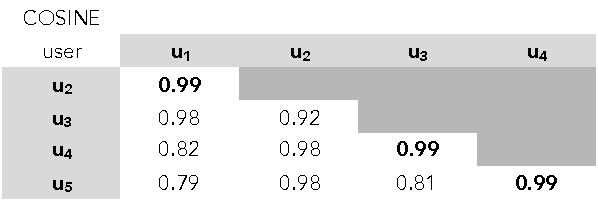
\includegraphics[width=\textwidth]{similarity_cosine.pdf}
        \caption{Cosine similarity}
        \label{table:cosine_similarity}
	\end{subtable}
    \vspace{10pt}

	\begin{subtable}[b]{0.55\textwidth}
		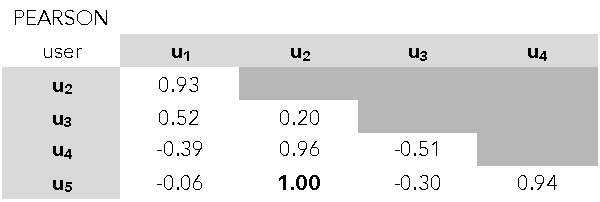
\includegraphics[width=\textwidth]{similarity_pearson.pdf}
        \caption{Pearson correlation}
        \label{table:pearson_similarity}
	\end{subtable}
    \vspace{10pt}
    
	\begin{subtable}[b]{0.55\textwidth}
		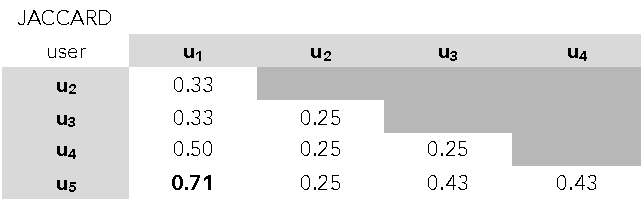
\includegraphics[width=\textwidth]{similarity_jaccard.pdf}
        \caption{Jaccard similarity}
        \label{table:jaccard_similarity}
	\end{subtable}
\end{table}
It can be seen that, according to the Cosine vector similarity metric (see Table \ref{table:cosine_similarity}), the most similar pairs of users are $(u_{1}, u_{2})$, $(u_{3}, u_{4})$, and $(u_{4}, u_{5})$, with a value of $.99$ each. On the other hand, the most dissimilar pairs of users are $(u_{1}, u_{5})$, $(u_{3}, u_{5})$, and $(u_{1}, u_{4})$, with values of $.79$, $.81$, and $.82$ respectively.
On the other hand, user similarity computed with Pearson correlation (see Table \ref{table:pearson_similarity}) estimates that the most similar pairs are $(u_{2}, u_{5})$, $(u_{2}, u_{4})$, and $(u_{4}, u_{5})$. 
It can be noticed that the user-pair $(u_{4}, u_{5})$ is the only pair that is ranked among the highest correlated pairs computed with the two metrics.
Also, $(u_{1}, u_{5})$ and $(u_{3}, u_{5})$ are among the less similar pair of users estimated by the two metrics. 
Contrarily, the similarity computed for the pair $(u_{3}, u_{4})$ differs greatly between the two methods. While Cosine vector estimates a high similarity for that user-pair, Pearson correlation returns a negative value of similarity. This is explained by the fact that the Cosine vector does not account for the mean or variances of the user's ratings, which in the case of users $u_{3}$ and $u_{4}$ are dissimilar. Pearson accounts for these differences and returns a different similarity value.
The Jaccard similarity metric (see Table \ref{table:jaccard_similarity}) estimates that the pairs of users $(u_{1}, u_{5})$ and $(u_{1}, u_{4})$ are the most similar ones. On the contrary, user-pairs $(u_{2}, u_{3})$, $(u_{2}, u_{4})$, $(u_{2}, u_{5})$, and $(u_{3}, u_{4})$,  are the most different. Moreover, these results differ from what was computed using Cosine vector and Pearson correlation due to the fact that Jaccard similarity does not consider the actual rating, but only the set of items for which there was preference, or interaction, between users. 

It is worth mentioning that neighbourhood approaches can be used not only to estimate similarities between users (given item agreement), but also to estimate similarities between items (based on users' ratings). User-user and item-item similarity estimation drive commercial user-based and item-based CF recommendation systems such as Amazon's ``Customers Who Bought This Item Also Bought'' and Amazon's ``Frequently Bought Together'' items, respectively \autocite{linden03amazon}.

Choosing a specific measure for computing similarity can greatly impact the estimated value of similarity. Pearson correlation can estimate a high similarity between users or items even if they have dissimilar rating values, or a low similarity even with similar  values. On the other hand, Cosine vector similarity can estimate that two vectors with same orientation but different magnitude are more similar than a pair of vectors with same magnitude but slightly different angle. All in all, different metrics lead to different estimations of similarity, and so choosing a specific one has a significant impact in neighbourhood-based recommendation. There is no consensus in which one is the best similarity metric, but most CF recommendation systems implement some of the aforementioned similarity metrics, Cosine vector and Pearson correlation in particular \autocite{leskovec14mining, ricci15recommender}.


One big disadvantage of using any of the aforementioned neighbourhood approaches for estimating similarities between users or items (and therefore for CF recommendation systems) is the need of initial rating data, otherwise the system will not know anything about a user and so it will be difficult to find like-minded people. 
Similarly, it would be difficult to recommend a new item entered into the database, because there have not been previous interaction with it.
Also, as the number of users and items increase, neighbourhood approaches suffer computational complexity since they have to estimate correlations between all pairs. 
Due to these shortcomings, the recommendation systems discussed so far have been abandoned since the late '90s and superseded by newer techniques based on learning models from the data.

\subsection{Model-based approaches}\label{sub:model} %or latent factor models, see \emph{koren08factorization}
A set of techniques for creating recommendations not based on finding the closest neighbours to users or items were developed later. These techniques aimed to improve the performance of recommendation systems by creating more accurate suggestions while diminishing the computational training time, thus allowing for manipulation of larger datasets \autocite{koren15advances}.
This series of techniques were called model-based recommendation methods by \textcite{breese98empirical}.

Model-based recommendation systems assume that CF recommendation can be viewed as a task of estimating the rating values of users on items not yet experienced.
Therefore, these systems learn a statistical model from the users' preferences, expressed as rating values in the utility matrix. The model is used afterwards to estimate the rating values that users would assign to items not yet experienced.

Using statistical and machine learning techniques, different  approaches have been used to design model-based recommendation systems. Cluster models and Bayesian network models were proposed and formalised by \textcite{breese98empirical}, linear regression was used by \textcite{sarwar01item} to learn models for predicting new ratings from past user ratings. \textcite{hofmann03collaborative} formalised a probabilistic approach for extracting latent classes from the data. Finally, \textcite{shani05mdp} had the hypothesis that the recommendation problem may be seen as a sequence of events that can be modelled by  implementing Markov decision processes in the context of a CF recommendation system. 

A review and description of the aforementioned as well as other model-based recommendation techniques was made by \textcite{adomavicius05toward}. 
The authors surveyed what they called the ``state-of-the-art'' in recommendation systems in the year 2005, defining a set of improvements that the next generation of recommendation systems should address in order to improve their recommendations.
However, the next big push in the development of new systems and approaches for recommendation came from the movie rental company Netflix. 


\subsubsection{The Netflix Prize}\label{sub:netflix}
% The movie subscription rental service \emph{Netflix} released in 2006 a dataset containing roughly 100M time-stamped ratings from 500K anonymous subscribers, on nearly 18K movie titles. The data reflected the distribution of all ratings (in a discrete scale) received by Netflix during a 7-year period. The whole dataset was divided into subsets for training, validation, and testing (96, 1.3, and 2.7 percent of the whole dataset respectively). 
%     Netflix challenged the research community to develop a recommender system capable of improving their own movie recommendation system by at least 10 percent, and offered a prize of one million dollar for the winner. Netflix's own recommendation system tried to predict the number of stars that a person would rate a video after watching it, on a scale from 1 to 5.
%     The improvement in accuracy should be computed using the RMSE of the system's prediction against the actual rating that a subscriber provides~\autocite{bennet07netflix}. 
In the year 2006, the DVD rental company Netflix challenged the research community to develop a system capable of improving the accuracy of Cinematch, their own proprietary recommendation system. The company offered a prize of one million dollar for the winner \autocite{bennet07netflix}.
 
Based on computing Pearson's correlation of users and movies, Cinematch determined a list of similar movies and predicted the rating a user would give to those items after watching them, on a scale from 1 to 5. 
In order to win the Netflix prize, a participating recommendation system should reduce by 10 percent the error that Cinematch computed between the actual subscriber movie rating and the prediction the participating system estimated for it. 
Participants were required to document and publish their approaches and findings publicly, thus encouraging researchers to benefit from the research of the other participants. 


To enable the contest, Netflix released a dataset containing roughly 100 million time-stamped ratings from 500K anonymous subscribers, on nearly 18K movie titles. The data reflected the distribution of all ratings (in a discrete scale) received by Netflix during a 7-year period. The whole dataset was divided into subsets for training, validation, and testing (96, 1.3, and 2.7 percent of the whole dataset respectively). 
However, research groups participating in the challenge only had access to the training and validation datasets. The testing dataset was used by Netflix for the evaluation of the submitted algorithms. 
The dataset, which was orders of magnitude larger than previously available datasets, provided the research community with the possibility to play with a very large dataset of user-item interactions. Exposing research groups to the actual demands of commercial recommendation systems could potentially lead to the development of new approaches to make better predictions, the development of new techniques to process the data, the discovery of trends and new insights from the data.
% training + probe set (training)
% qualifying set = quiz(50%)+test(50%)



During the first year of the contest, more than 20K teams were registered for the competition and more than two thousand actually submitted their predictions. An online leaderboard managed by Netflix registered all submissions, their results, and links to their webpages and publications.\footnote{The leaderboard of teams, their marks, and link to their publications is still available at \url{http://netflixprize.com/leaderboard.html}} However, after the first year none of the submissions achieved the improvement in accuracy required to win the prize; the leading research groups reached a plateau at about 7 percent of accuracy improvement.

Since there was no winner, the competition went on for another year and a half. Due to the requirement for the research groups to publicly document their procedure and report all findings, some of the participating teams started to discuss and share code, coding ideas, and insights from the patterns found in the data. Furthermore, some of these teams started to work together in order to combine and blend their implementations to achieve the required increase in accuracy.

Finally, two teams submitted their predictions and achieved an improvement of 10.06 percent each by the due date in July 2009. Despite they achieved the same result, the winner team submitted their solution 20 minutes before the second-place team. The Grand prize went to the team named ``BellKor's Pragmatic Chaos,'' which was a combination of the teams ``BellKor'' and ``Big Chaos''\autocite{koren09bellkor}, teams that were in top of the leaderboard ranking in previous years.

One of the big insights that the Netflix competition provided was that no single unique recommendation algorithm could achieve the desired improvement in accuracy. As a result, teams had to join forces---their algorithms, methods, and insights learned from the data---in order to reach the mark. Therefore, after three years of work, the aforementioned two teams beat the challenge by combining several teams' ideas and algorithms into more complex models that made possible to improve the accuracy of their predictions.
% For example, ``BigChaos'', one team of the winning team, devised a three-dimensional model that incorporated time into the relationship between people and movies. 
The ``BellKor's Pragmatic Chaos'' team developed and implemented hundreds of models to represent the data that Netflix released. Then, they used an iterative process of optimization by which the algorithm with the lowest contribution to increase the overall accuracy of the system was removed in each iteration. In the end, 18 predictors were used to achieve the goal of obtaining the 10 percent accuracy improvement \autocite{toscher09bigchaos}. 

The Netflix prize competition demonstrated that model-based approaches achieved a better performance and are more scalable for large datasets than nearest neighbour-based techniques \autocite{koren09matrix}. The winning model-based approaches used in the competition were based on finding a set of latent factors that explained the ratings of items by users. In particular, the latent factor technique that achieved the best performance in terms of accuracy and scalability for the data of the competition was matrix factorization. 
In the next subsection, we review and describe how matrix factorization is used to approximate the rating matrix. This process is driven by finding a set of factors inferred from the rating patterns that characterise some intrinsic, to-be-revealed aspects of users and items, which can then be used to estimate the ratings of users in items not yet experienced.

% Among various collaborative recommendation techniques, model-based approaches are more scalable than memory-based approaches for large scale data sets in spite of large offline computation and difficulty to update the model in real time.




\subsection{Matrix factorization}\label{sub:matrix}
% Check \url{http://www.quuxlabs.com/blog/2010/09/matrix-factorization-a-simple-tutorial-and-implementation-in-python/}
While previously described neighbourhood-based methods for recommendation are intuitive and their results easy to interpret, matrix factorization techniques allow to discover underlying latent factors between the interaction of users and items. 
Matrix factorization is a mathematical technique for reducing the dimensionality of a matrix. Any matrix can be approximated by finding two or more matrices that, when multiplied, reconstruct closely the original matrix. Therefore, the goal in matrix factorization is to compute a set of lower-dimensional matrices that approximate the original rating matrix. 

In the context of recommendation, the rows of the estimated low dimensional matrices can be interpreted as a set of latent factors that determine partially the reaction of users to items. Then, the values of these latent factors are used to predict the preference of users on those items not yet rated.
That is, the estimated latent factors can be visualised as the items' features that cause people's preference on them \autocite{koren09matrix}. 
% In other words, 



Since each user typically only interacts with a very small subset of items from the complete available collection, the utility matrix is very sparse (in numerical analysis, a sparse matrix is a matrix in which most of the elements are zero, null, or have an empty value. By contrast, if most of the elements are nonzero, then the matrix is considered dense). This tendency creates problems for neighbourhood-based approaches because it leads to poor estimations of similarity. With matrix factorization, the sparsity of rating matrices is addressed by projecting users and items into a reduced latent factor space that captures the most salient features of the dataset \autocite{ricci15recommender}.

Formally, all user-item interactions in the rating matrix can be modelled as inner products in a joint latent feature space with dimensionality $f$.
Each item $i$ is associated with a vector $\boldsymbol{q}_i \in {\rm I\!R^f}$, and each user with a vector $\boldsymbol{p}_q \in {\rm I\!R^f}$.
For each item $i$, values in $\boldsymbol{q}_i$ represent to which extent the item possesses those latent characteristics. On the other hand, for each user $u$, values of $\boldsymbol{p}_u$ embody how much the user pays attention to those latent features. 
The dot product of the arrays  accounts for the interaction between each user's interests on each item's characteristics. This product approximates the rating $\boldsymbol{r}_{ij}$ of user $u$ on item $i$, and leads to the estimated rating:
\begin{equation}
% \vspace{-2em}
\hat{\boldsymbol{r}}_{ij} = {\boldsymbol{q}_i}^T \boldsymbol{p}_u
\end{equation}

Yehuda Koren, who led ``BellKor's Pragmatic Chaos,'' the team that won the Netflix  Prize competition, stated conceptually the matrix factorization approach for recommendation and also detailed its implementation in a number of publications \autocite{koren08factorization, koren09collaborative, koren09matrix, koren15advances}. 
In these publications, Koren explained that the preferences expressed by users for items can be biased due to the tendency of users to use the preference scale differently. This might lead to some users rating items in a more extreme way than others, or having some items that are rated higher than others. Thus, biases on users' item ratings should be taken into account and removed when doing the estimation of the latent factor values. 

In the process of normalisation, input values are transposed to a common scale by removing the overall matrix mean, as well as row and column means. In other words, the mean of users and items, respectively. After the normalisation process, a model based on latent factors tries to learn the factor vectors $\boldsymbol{r}_{ui}$ by means of minimizing the square error from the set of known ratings. 

The process of minimizing the error can be formalised as follows, with $\mathcal{K}$ being the set of $(u,i)$ pairs for which $\boldsymbol{r}_{ui}$ is known:
\begin{equation}
\min_{\boldsymbol{q}, \boldsymbol{p}} 
\displaystyle\sum_{(u,i) \in \mathcal{K}} 
(\boldsymbol{r}_{ui} - {\boldsymbol{q}_i}^T \boldsymbol{p}_u)^2 
% \vspace{1em}
\end{equation}

Moreover, in order to minimise the risk of overfitting the training data, a regularization parameter is used to control the magnitudes of the learned factors \autocite{bell07scalable}.
This regularization parameter is called the lambda value, and is chosen by comparing the prediction error between the training and testing datasets. The higher the value of lambda, the more is the regularization applied. What constitutes an appropriate lambda value is dependant on the size, characteristics, and sparsity of the underlying data. A sensible value for lambda should be the one computing a similar error value for the two sets. Hence, this regularization parameter is data-dependant and can not be chosen in advance, it should be tuned using out-of-sample test data.
The final expression for learning the factor vectors considering the regularization is therefore expressed as:
\begin{equation}
\min_{\boldsymbol{q}, \boldsymbol{p}} 
\displaystyle\sum_{(u,i) \in \mathcal{K}} 
(\boldsymbol{r}_{ui} - \boldsymbol{q}_{i}^T \boldsymbol{p}_u)^2 
+ \lambda(\|\boldsymbol{q}_i\|^2 + \| \boldsymbol{p}_u \|^2)
% \vspace{1em}
\end{equation}




To find the best values for $\boldsymbol{p}$ and $\boldsymbol{q}$ that minimise the error in those  entries where $\boldsymbol{r}_{ui}$ is non blank, learning optimization algorithms such as gradient descent or alternating least squares are usually implemented. 
In stochastic gradient descent, matrices are initialised with a set of values and the difference between all predicted ratings and actual ratings is calculated, in what is known as prediction error. Then, the values of the matrix are modified by a small amount, searching for the change of direction that makes the prediction error smaller. This process is repeated iteratively,  most of the time converging to a minimum value \autocite{funk06netflix}.

On the contrary, instead of optimizing values of factors for users and items at the same time, the alternating least squares approach rotates between fixing one set of values and then the other. Once the values for a set of features are fixed, their counterparts are minimised by solving a least-squares problem, and vice-versa. This iterative process is repeated until converging when no significant improvement is achieved \autocite{bell07modeling}.

As these optimization processes are stochastic, the final values are not always the same, however they usually tend to be close. A common approach that avoids predicting merely one possible set of values is to run the process several times and use the mean value of all computed latent factor values as the resultant ones.












% \subsubsection{Synthetic data example}

% In order to understand how matrix factorization can help to uncover latent features from the data, we present a synthetic example with a small amount of data describing people's ratings on tracks.

% In our example, a set $U$ of 32 users have expressed their preference on a set $V$ constituted by 16 tracks.  
% Three synthetic control features represent aspects of the music tracks:  \emph{tempo}, \emph{vocalness}, and \emph{electronicness}. Users were split in eight balanced groups of preferences, with four people each.
% We generated ratings for the set of users $U$ considering how much they preferred those control features. Rating values were randomly chosen between 4 and 5 in a 5-level Likert scale for the preferred tracks.  Non-preferred received a value of 1. 

% We used matrix factorization to find a set of matrices that, when multiplied, approximate the original rating matrix. We chose $k = 3$ latent factors and estimated a set of two low-rank matrixes that approximated the ratings of the original matrix.
% The error found of the reconstructed matrix was 0.91, meaning that the estimated ratings were away from the actual, original rating by less than one Likert level in average.

% Fig.~\ref{fig:toy_example_comparison} shows the original and the reconstructed matrix of ratings for all users and tracks. Fig.~\ref{fig:original_rating_matrix} shows the original rating matrix. The eight groups of users can be seen clearly clustered according to their preferences on the control features. Fig.~\ref{fig:reconstructed_rating_matrix} shows the reconstructed rating matrix. It can be seen that although the matrix was only partially reconstructed, perhaps due to the low number of latent factors chosen or the data topology, many zones of the reconstructed version resemble the original matrix and the eight different groups of users can be visualized. 


% \begin{figure}[ht!]
% 	\centering
% 	\begin{subfigure}[b]{0.75\textwidth}
% 		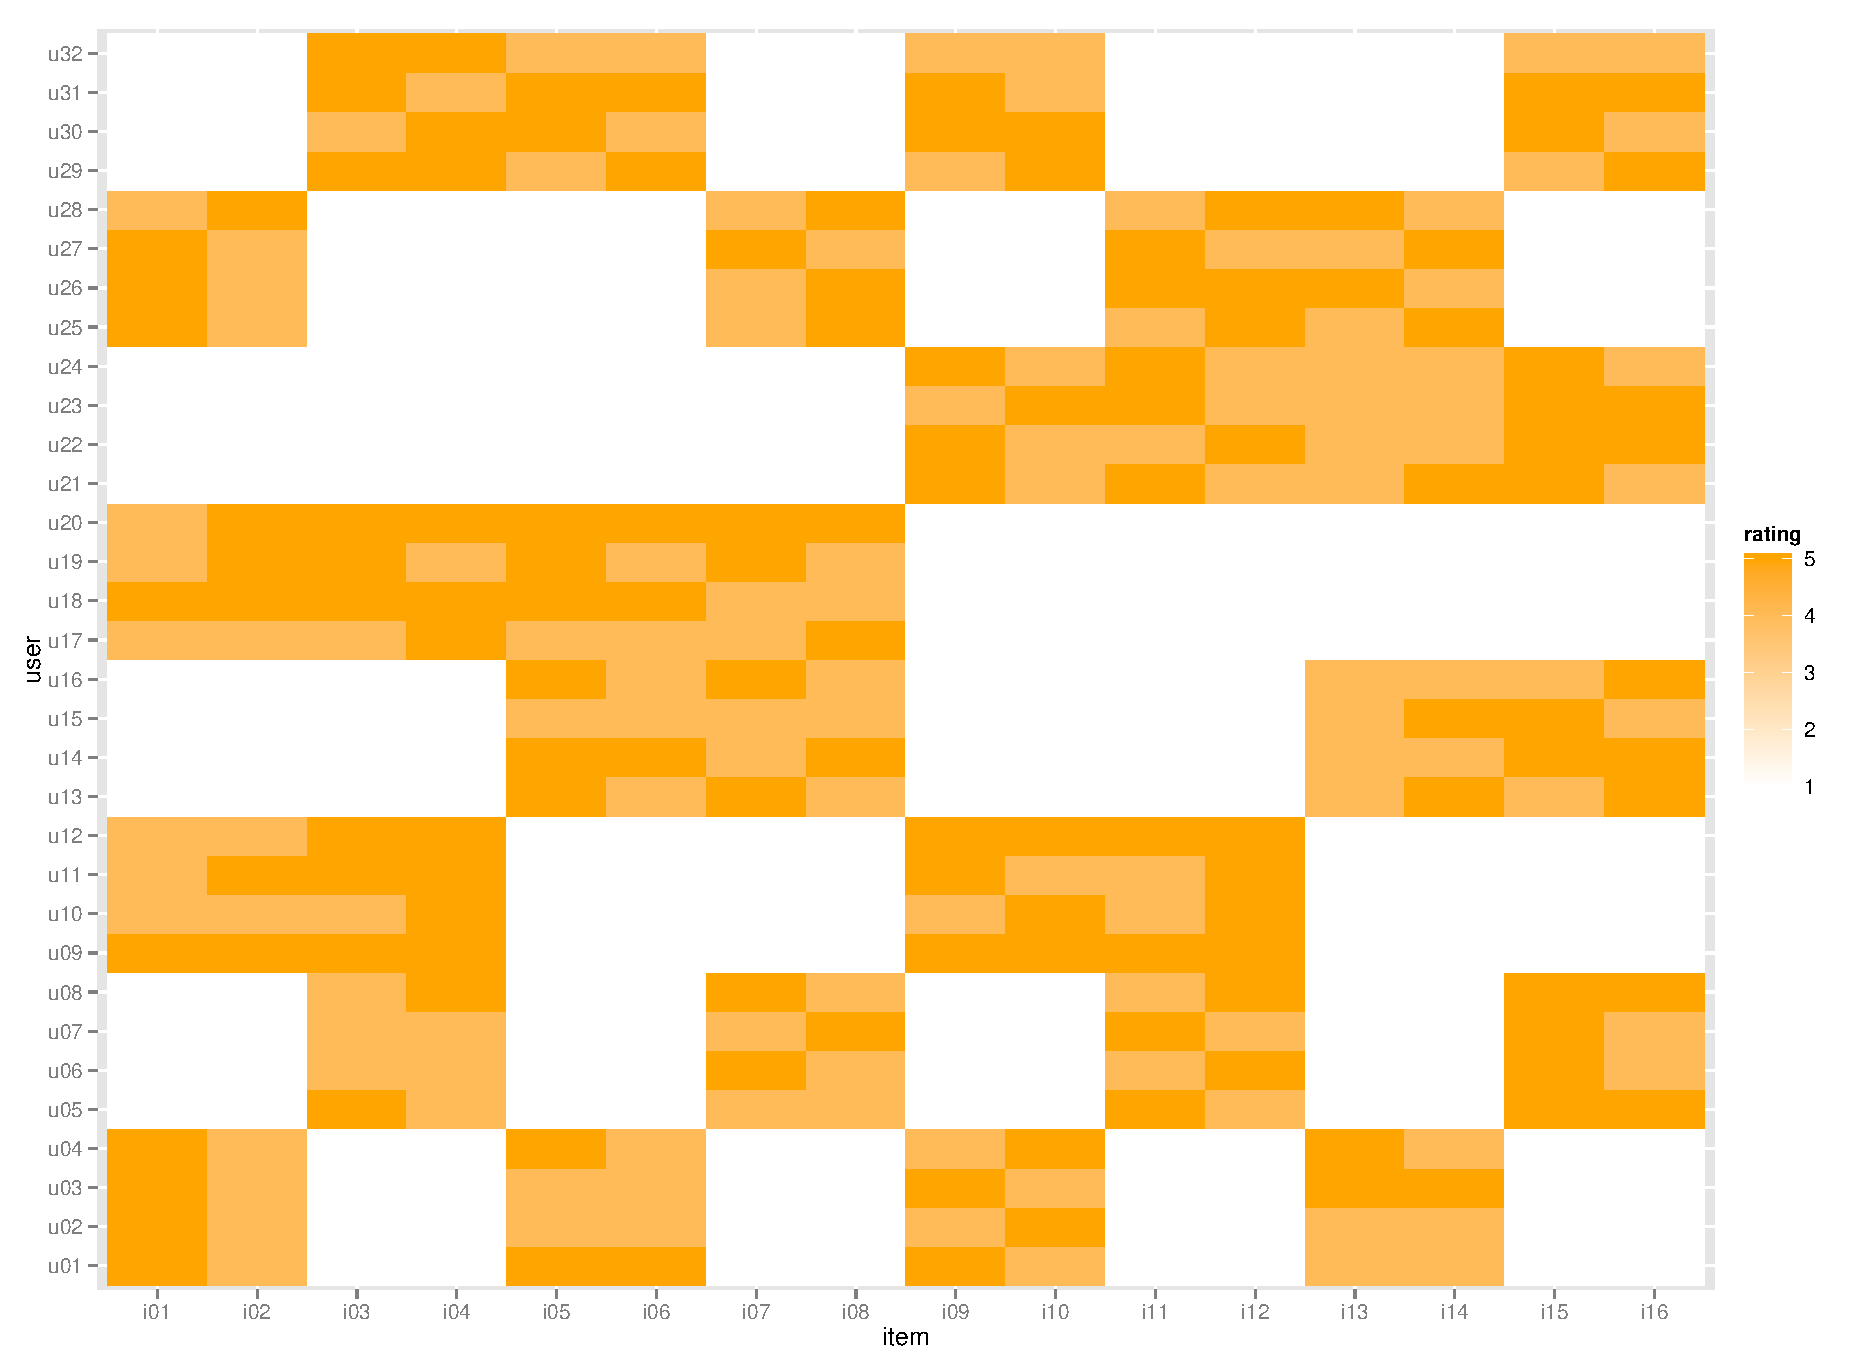
\includegraphics[width=\textwidth]{toy_example_32_users_16_item_8_groups_rating_matrix.pdf}
%         \caption{Original rating matrix with synthetic data}
%         \label{fig:original_rating_matrix}
% 	\end{subfigure}
%     \vspace{10pt}

% 	\begin{subfigure}[b]{0.75\textwidth}
% 		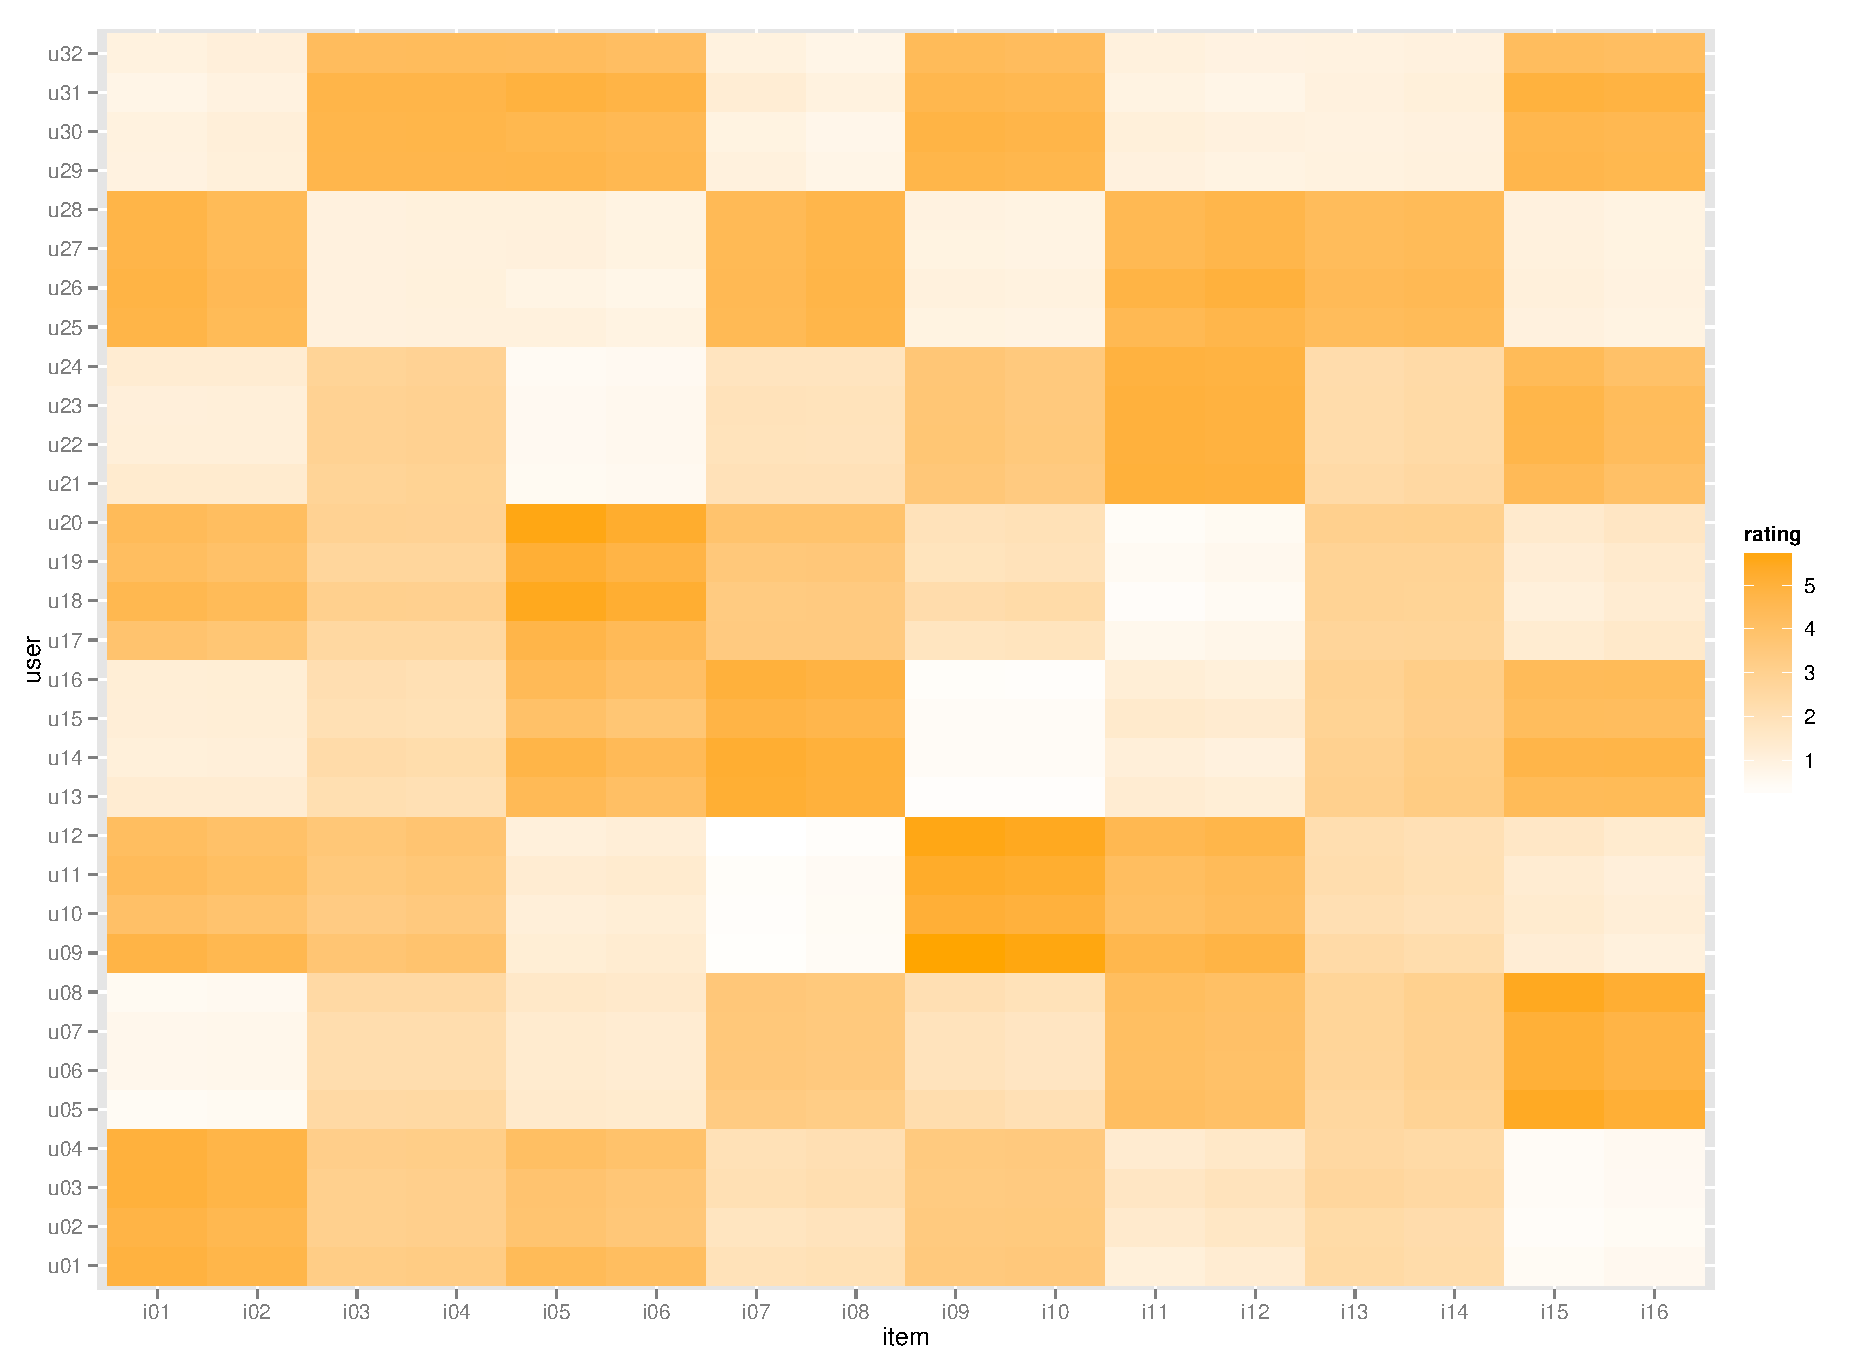
\includegraphics[width=\textwidth]{toy_example_32_users_16_item_8_groups_rating_matrix_reconstruction_3_factors.pdf}
%         \caption{Reconstructed rating matrix}
%         \label{fig:reconstructed_rating_matrix}
% 	\end{subfigure}
%     \vspace{10pt}
    

% \caption{Original and reconstructed rating matrixes of synthetic data example with 32 users expressing their preference on 16 tracks.}
% \label{fig:toy_example_comparison}
% \end{figure}






% \begin{figure}[ht]
% \vspace{1em}
% \centering
% 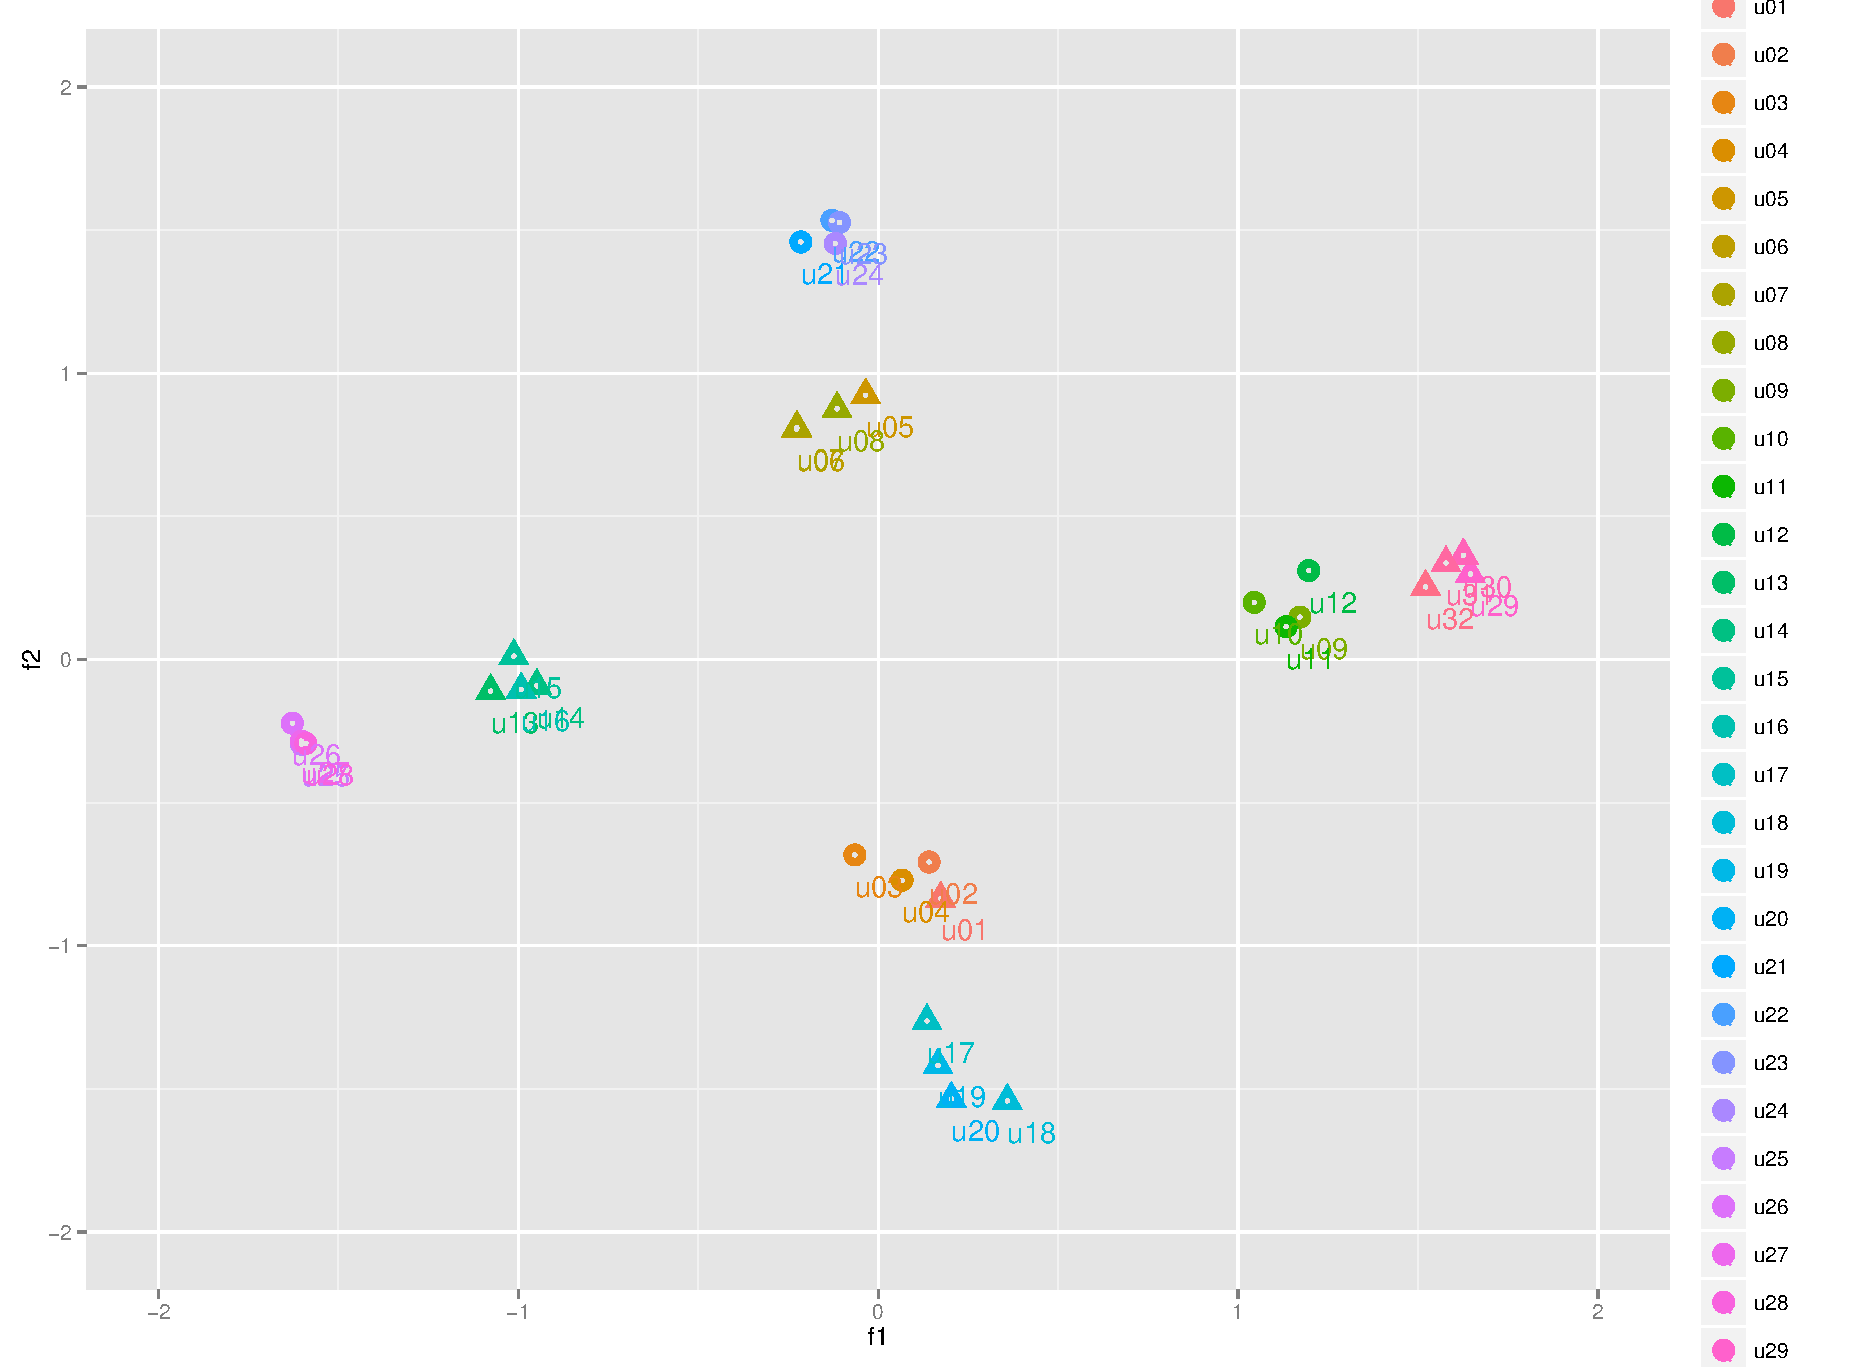
\includegraphics[width = 1\textwidth]{toy_example_32_users_16_item_8_groups_users_mf_3factors.pdf}
% \caption{Latent factor plotting for users in toy example }
% \label{fig:preference-toy-example-users-8-categories-3factors}
% \end{figure}

% We also plotted the values of the two estimated low-ranking matrixes. 
% Fig.~\ref{fig:preference-toy-example-users-8-categories-3factors} shows the values for the three latent factors for all users in the dataset.
% The visualisation shows that the distribution of users in the three latent factors follow a certain pattern. 

% Each group clusters users that have rated similarly tracks they prefer, according to the synthetic features described before. 
% All subgroups of users that are in opposite quadrants within the plot, i.e., 
% $\{u_{01}, \ldots,  u_{04}\}$ and $\{u_{05}, \ldots, u_{08}\}$,
% $\{u_{09}, \ldots,  u_{12}\}$ and $\{u_{13}, \ldots, u_{16}\}$, 
% $\{u_{17}, \ldots,  u_{20}\}$ and $\{u_{21}, \ldots, u_{24}\}$, and
% $\{u_{25}, \ldots,  u_{28}\}$ and $\{u_{29}, \ldots, u_{32}\}$, 
% are the less similar sub-group of users, which is expected since they do not share any preferences. 
% Groups of users that share more preferences, are closer in space. 

% On the other hand, Fig.~\ref{fig:preference-toy-example-items-8-categories-3factors} shows how items are projected in a three-factor latent space, where the third axis $f3$ is expressed as being in the positive or negative side of the $f1$ and $f2$ plane. 
% It can be seen that items that were preferred similarly are placed close to each other in space. Also, item pairs that are further apart are the ones that share less preferences by users. Some item pairs, such as
% $\{i_{01}, i_{02}\}$ and $\{i_{05}, i_{06}\}$, and
% $\{i_{11}, i_{12}\}$ and $\{i_{15}, i_{16}\}$
%  are in opposite sides $\{+, -\}$ of the third axis, and so they are further apart to what is apparently seen in the plot. This characteristic indicates that these items share only some features. 

% Interestingly, a mapping can be established from preferences expressed by users between the set of synthetic dimensions and the three latent factors. Item pairs
% $\{i_{03},  i_{04}\}$ and $\{i_{09}, \ldots, i_{10}\}$ lie in the same octant. 






% \begin{figure}[ht]
% \vspace{1em}
% \centering
% 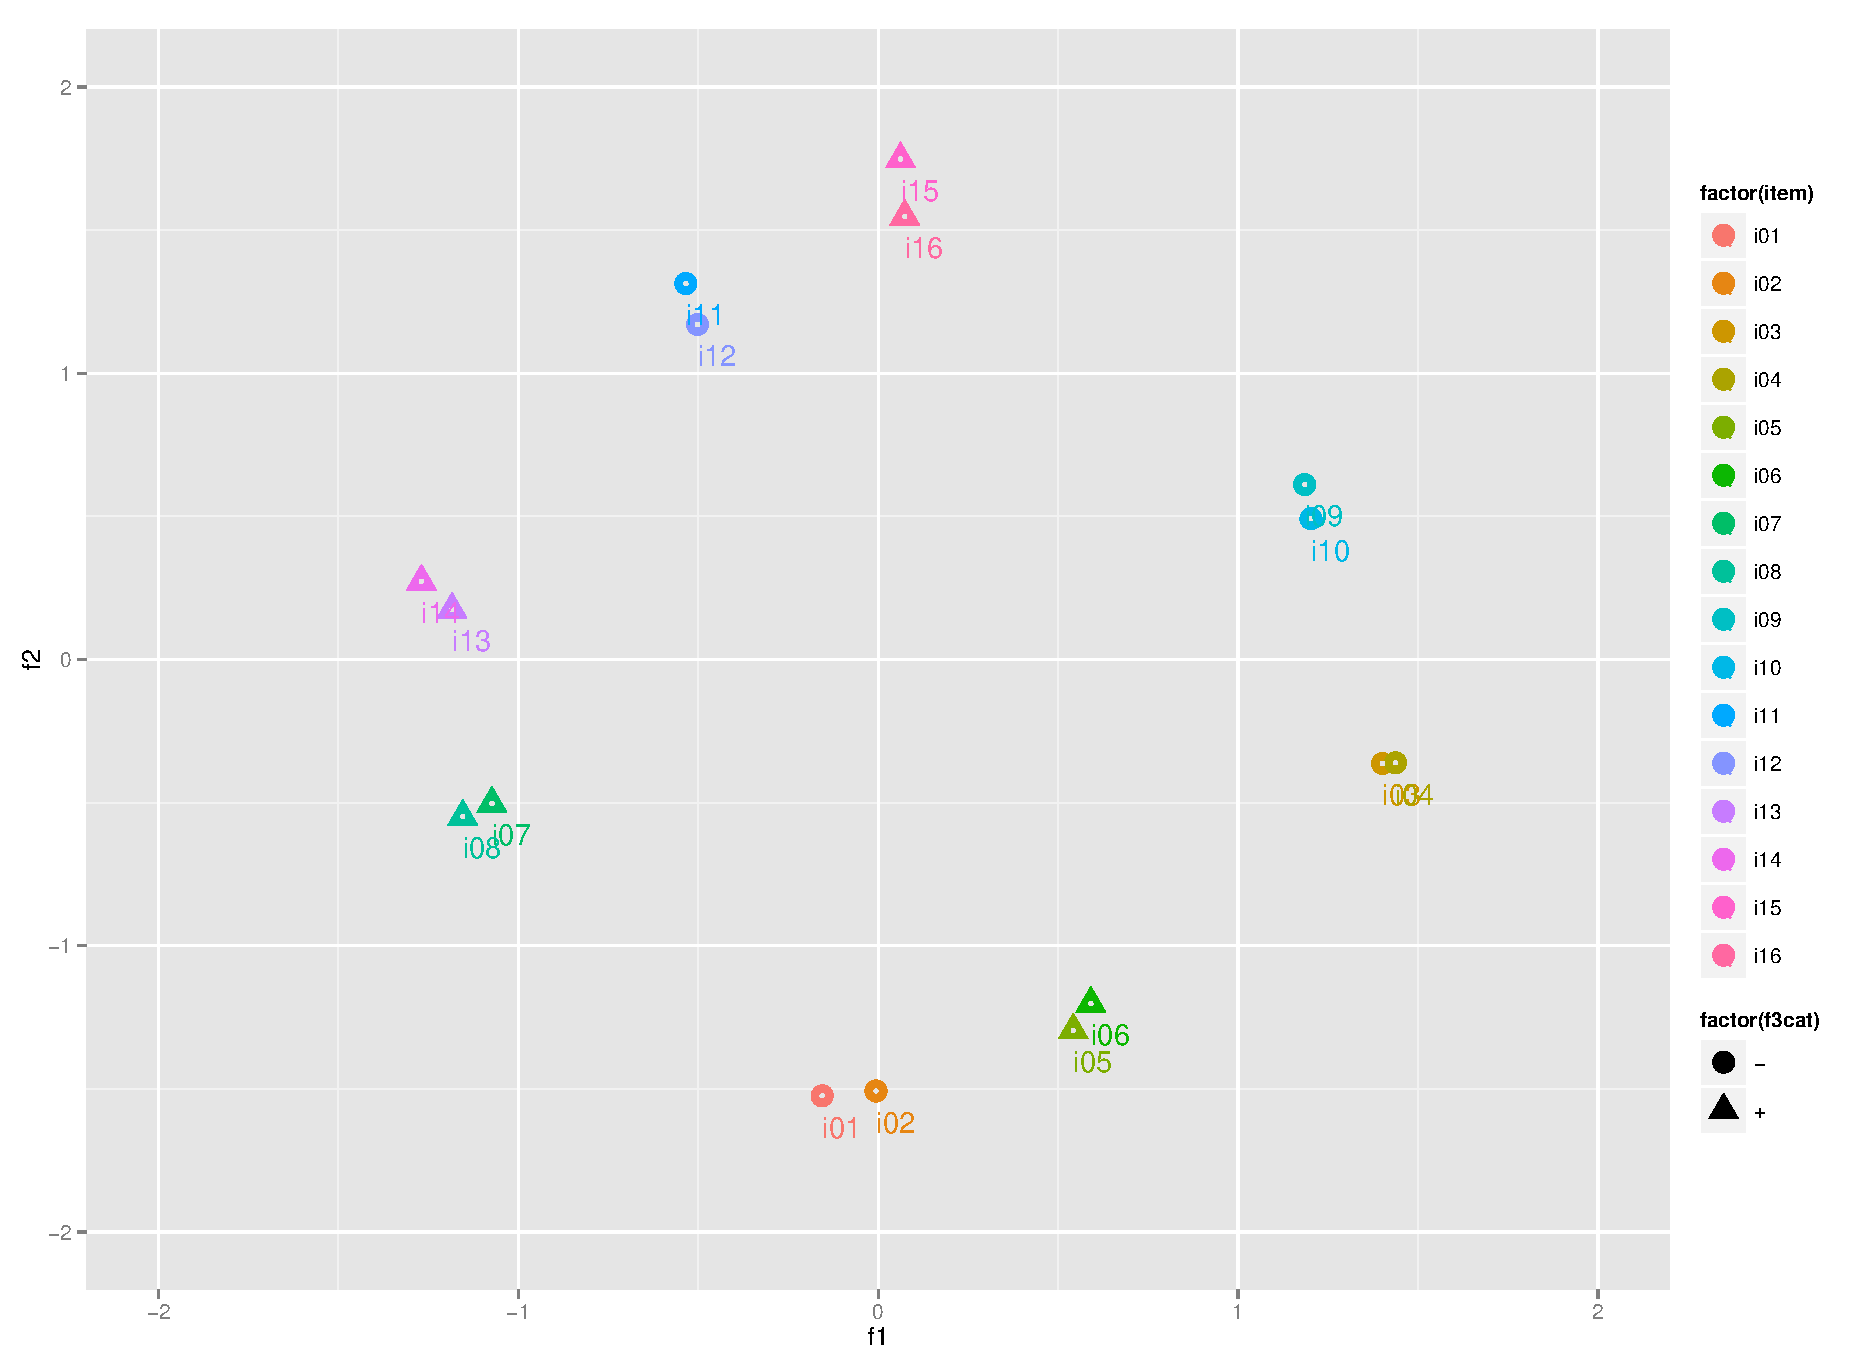
\includegraphics[width = 1\textwidth]{toy_example_32_users_16_item_8_groups_items_mf_3factors.pdf}
% \caption{Latent factor projection of items in synthetic example }
% \label{fig:preference-toy-example-items-8-categories-3factors}
% \end{figure}



% Fig.\ref{fig:Iconic_artists_2dim_allusers_2} shows how artists, from a set of iconic artists, gets positioned in a two-dimensional plot according to the extracted values for two latent features using data from 590K users, with regularization parameter 1e-07, and 50 iterations. 
% It is interesting noting that artists that usually are considered as related-artists, are close neighbours in this 2-dimensional latent factor space. For example, while the lower right quadrant has mainly artists related to metal rock, mostly all female artists are located in the upper right quadrant. On the other hand, while the lower left quadrant has artists with characteristics of repetition or introspection, artists in the upper left quadrant are more extrovert.
% This distribution of artists resembles to the circumplex model of affect with
% arousal and valence dimensions \autocite{russell80circumplex}. The y-axis might be interpreted as the level of \emph{arousal}, where artists in the lower part have lower arousal. On the other hand, the x-axis seems to be related to \emph{valence}. 



% \begin{figure}[ht]
% \vspace{1em}
% \centering
% 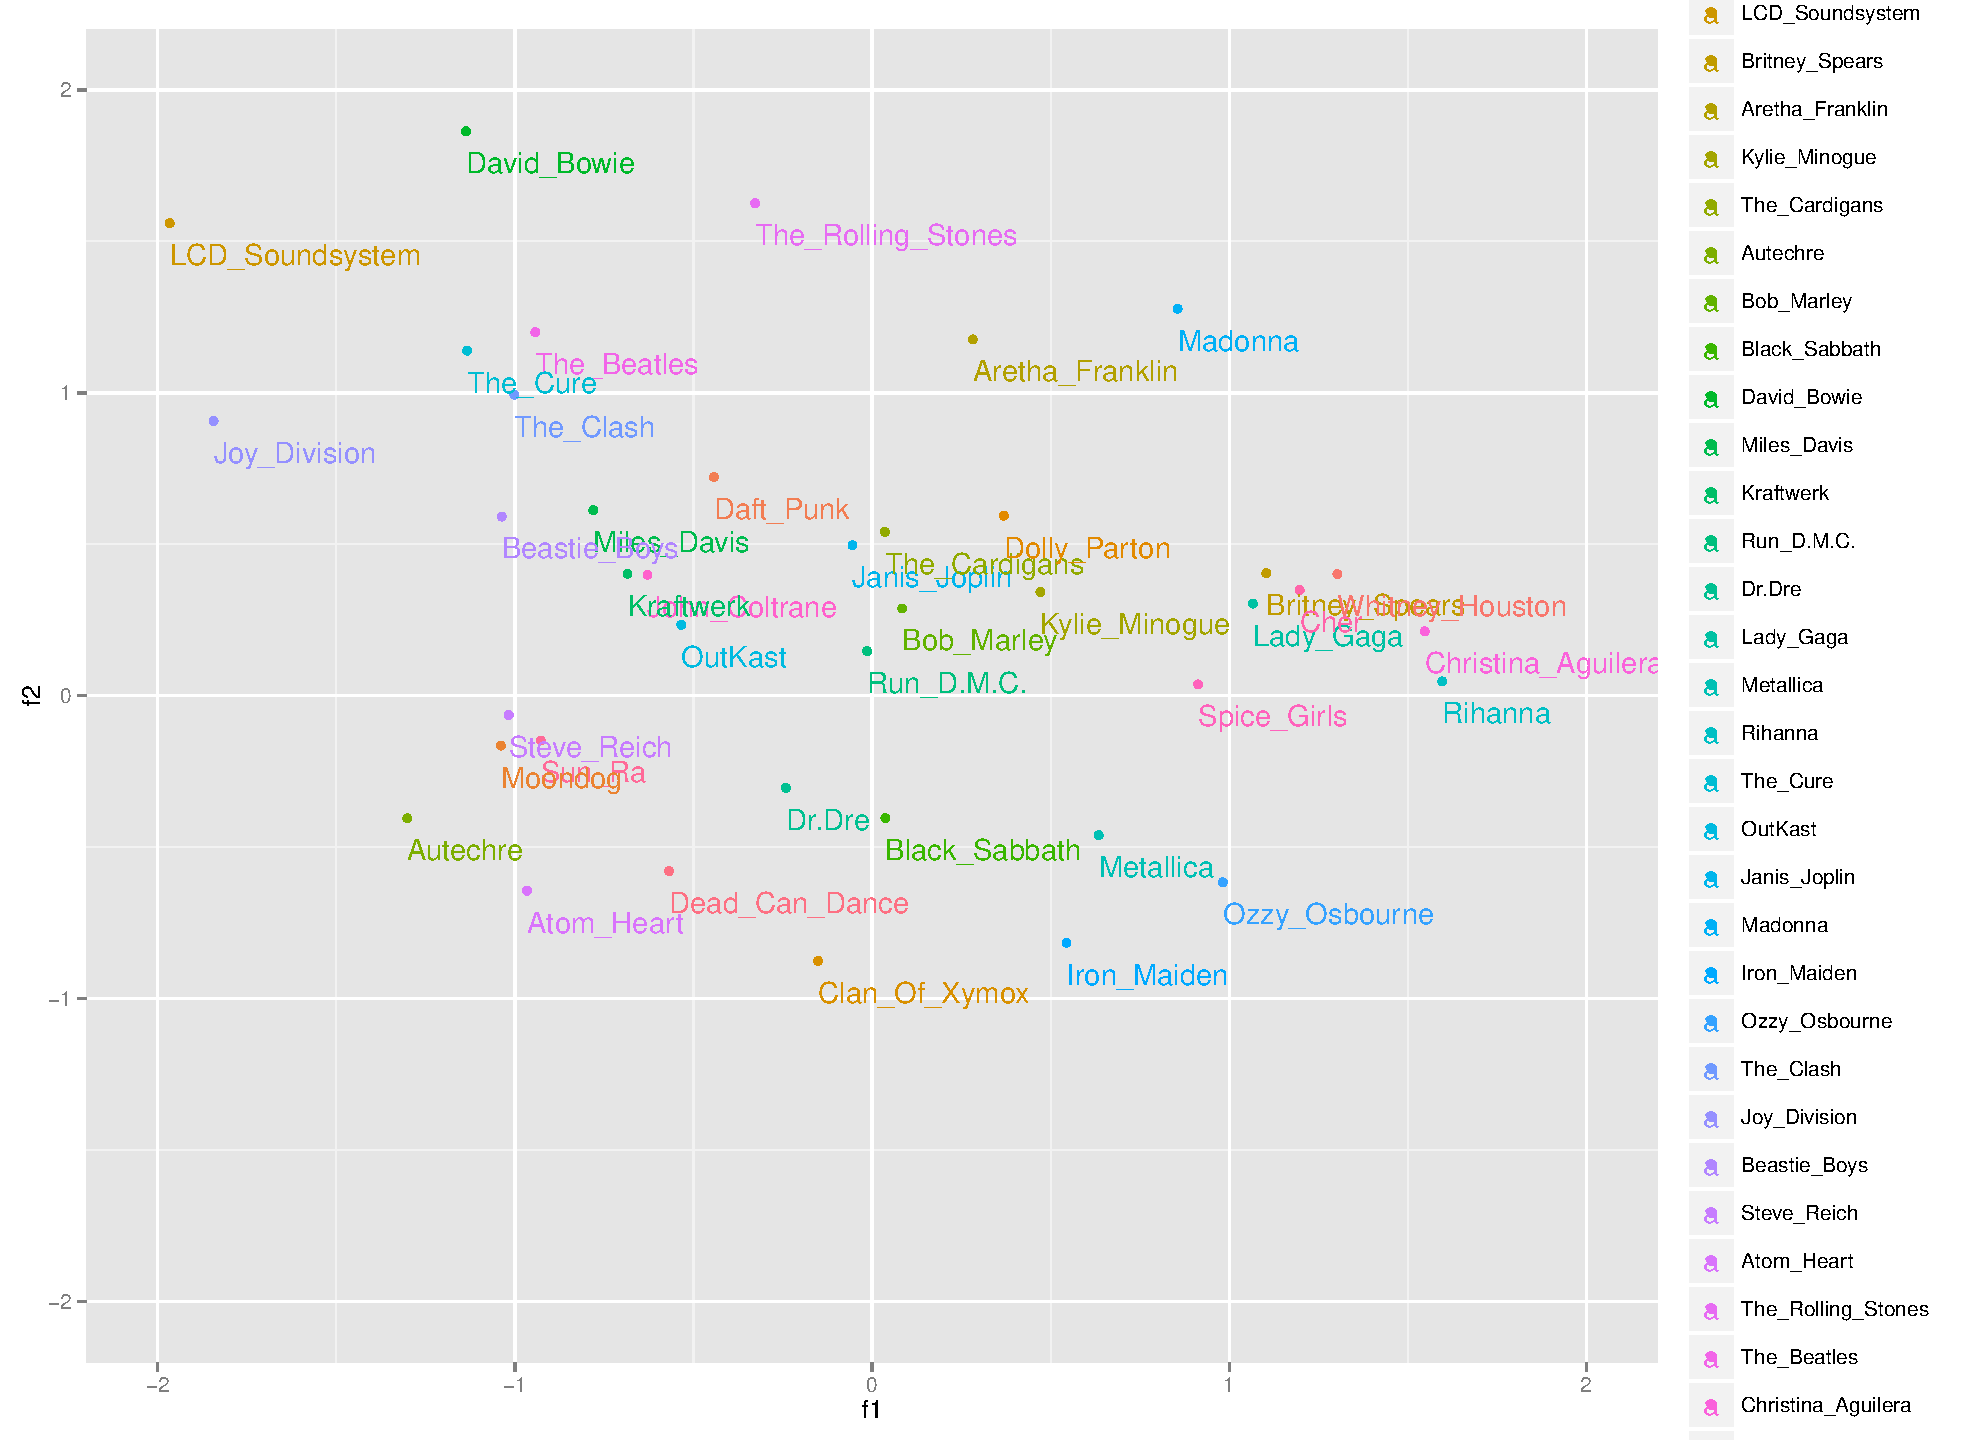
\includegraphics[width = 1\textwidth]{iconic_artists_2.pdf}
% \caption{Latent factor plotting for set of iconic artists }
% \label{fig:Iconic_artists_2dim_allusers_2}
% \end{figure}
















% \subsection{Factorization machines}\label{sub:factorization_machines}
% \emph{Factorization machines} \autocite{rendle10factorization} is a general method for approximating a target matrix based on matrix factorization, however it is also able to incorporate as part of the prediction model a set of side data features. 
% Hence, instead of just estimating a user-defined number of latent factors for approximating a preference matrix, user- and item-side data can be also included to approximate the observed preference ratings. 

% The estimated side-data values can also be used to predict preference of users on items even when there are no observed preferences, just by considering the user and item side-data. For example, when a new user registers herself in a music streaming service there is no previous listening history data for that listener, and so demographic data might be used to recommend the best artist or tracks for that specific user, in relation to how listeners with similar demographic characteristics have expressed preferences on music items.

% On top of incorporating more data in the model, \textcite{rendle10factorization} also claimed that factorization machines are able to estimate parameters of the model under very sparse data, common case in collaborative filtering recommendation where users have expressed preference for a minute part of the dataset of items. 
% The author also demonstrates that the numeric complexity of the model is linear in terms of the dimensionality of the factorization and the number of variables, meaning that they are easily scalable to large dataset. Factorization machine models are also able of expressing categorical and real-valued data.

% The factorization machine model was formalized by \citeauthor{rendle10factorization} as:

% \begin{center}
% \vspace{1em}
% \label{eq:factorization_machines_formalization_1}
% $
% \hat{y}(x) := w_{0} + \displaystyle\sum_{i=1}^{n}w_{i}x_{i} + 
%  	\sum_{i=1}^{n}\sum_{j=i+1}^{n}
%  	\langle \vec{v_{i}},\vec{v_{j}}\rangle x_{i}x_{j} 
% $
% \end{center}


% where model parameters to be estimated are

% \begin{center}
% \vspace{1em}
% \label{eq:factorization_machines_formalization_2}
% $
% w_{0} \in \mathbb{R}, \vec{w} \in \mathbb{R}^{n}, \vec{V} \in \mathbb{R}^{n\times k}
% $
% \end{center}

% and $\langle \vec{\cdot},\vec{\cdot}\rangle$ is the dot product of vectors of size $k$:

% \begin{center}
% \vspace{1em}
% \label{eq:factorization_machines_formalization_3}
% $
% 	\langle \vec{v_{i}},\vec{v_{j}}\rangle :=
% 	\displaystyle\sum_{f=1}^k{v_{i,f}\cdot v_{j,f}}
% $
% \end{center}

% $w_{0}$ corresponds to the global bias term, which can be understood as the average rating value that is surrounded by all other ratings. $w_{i}$ are the weight terms of the $i$-th variable. $\langle \vec{v_{i}},\vec{v_{j}}\rangle$ models the interaction between all latent factors. 

% To exemplify the use of factorization machines, a toy example is described now. A small set of listeners have expressed their preferences on a set of ten artists. Each listener have expressed preference on a subset if artists. Also, one of the listener has not expressed preference on any item. There is categorical information about the gender and age for each listener.~\ref{fig:six_users_factorization_machines_1} shows the preference matrix for all users and artist in the toy dataset.


% \begin{figure}[ht]
% \vspace{1em}
% \centering
% 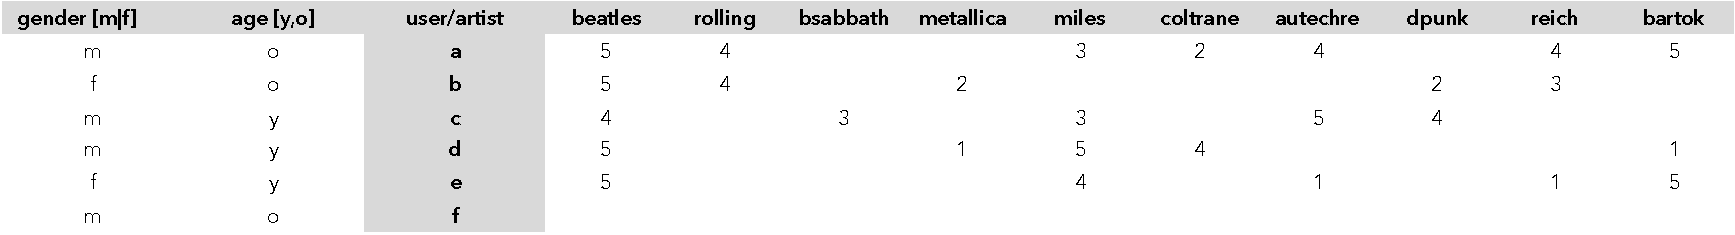
\includegraphics[width = 1.0\textwidth]{six_users_factorization_machines_1.pdf}
% \caption{Preference matrix for a small set of listeners with categorical data on a set of artists.}
% \label{fig:six_users_factorization_machines_1}
% \end{figure}

% By using the factorization machines method, we try to estimate a set of optimal values for the user-defined number of latent factors for users, items, and all side data that minimize the error when reconstructing the matrix of preferences.
% This method not only estimates latent factors for users and items, but also for each side data variable, along with the global bias term, and the linear intercepts for each variable. For estimating the optimal values, not only the interaction between latent factor of users and items are considered, but the interaction between the latent factors of all variables. In the toy example case, this implies the interaction between $\langle user, item\rangle$, $\langle user, gender\rangle$, $\langle user, age\rangle$, $\langle item, gender\rangle$, $\langle item, age\rangle$, and also $\langle gender, age\rangle$.

% Fig.~\ref{fig:six_users_factorization_machines_2} and Fig.~\ref{fig:six_users_factorization_machines_3} show the estimated values for the global bias term, and biases for all users, items, and side features, as well as the values for two two latent factors. 


% \begin{figure}[ht]
% \vspace{1em}
% \centering
% 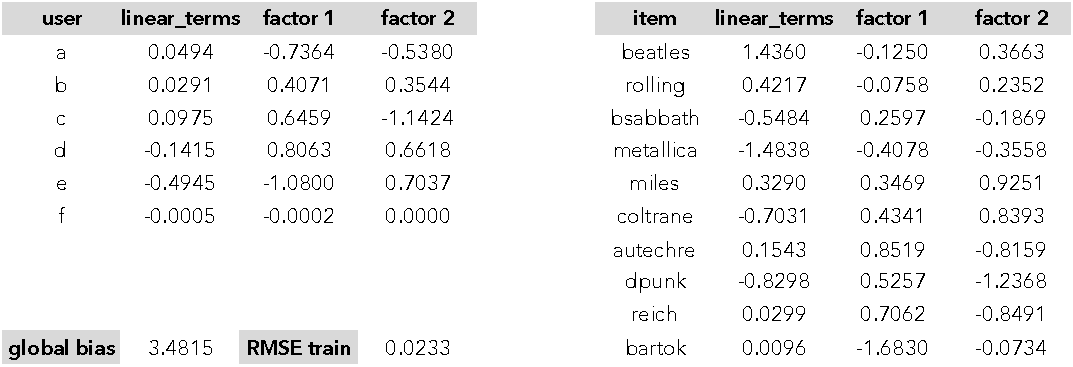
\includegraphics[width = 0.9\textwidth]{six_users_factorization_machines_2.pdf}
% \caption{Estimated latent factors for users and items}
% \label{fig:six_users_factorization_machines_2}
% \end{figure}


% \begin{figure}[ht]
% \vspace{1em}
% \centering
% 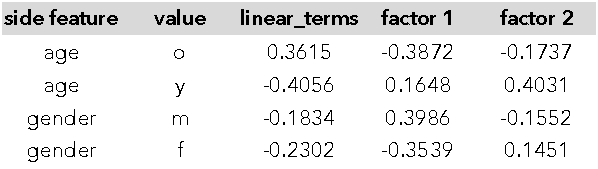
\includegraphics[width = 0.5\textwidth]{six_users_factorization_machines_3.pdf}
% \caption{Estimated latent factors for user side data}
% \label{fig:six_users_factorization_machines_3}
% \end{figure}

% As can be seen, values for all expressed preferences have been correctly reconstructed and values for unobserved preferences have been estimated. Even so, a set of ratings for user $f$, which did not have any expressed preference on any music item, has been estimated. 
% The computation of every single value has considered the global bias, the biases for each user, item, and side features, and the interaction between the latent factors of all these variables. 
% Interestingly, it can be seen that the bias for user $f$, as well as the latent two factors, are very close to zero. This makes sense since there is no previous music preference information about this zero. The only known feature variables for this user are his gender (male), and his age bracket (old). 
% Hence, just to clarify the computation of a single predicted value, the estimation of the preference of user $a$ in the artist John Coltrane (JC) is computed by:

% % Global bias term + bias user $a$ + bias item $John Coltrane$ + interactions between all variables

% \begin{center}
% \vspace{1em}
% \label{eq:matrix_factorization_formalization_test}
% $
%  Global\ bias\ term + bias_{user(a)} + bias_{item(JC)} +\newline
%  f1_{user(a)}\cdot f1_{item(JC)} + f2_{user(a)}\cdot f2_{item(JC)} +\newline
% f1_{user(a)}\cdot f1_{gender(user(a))} + f2_{user(a)}\cdot f2_{gender(user(a))} +\newline
% f1_{user(a)}\cdot f1_{age(user(a))} + f2_{user(a)}\cdot f2_{age(user(a))} +\newline
% f1_{item(JC)}\cdot f1_{gender(user(a))} + f2_{item(JC)}\cdot f2_{gender(user(a))} +\newline
% f1_{item(JC)}\cdot f1_{age(user(a))} + f2_{item(JC)}\cdot f2_{age(user(a))} +\newline
% f1_{gender(user(a))}\cdot f1_{age(user(a))} + f2_{gender(user(a))}\cdot f2_{age(user(a))}
% $

% \end{center}

% Hence, in the case of the synthetic example, the computed preference of user $a$ in the artist John Coltrane is 2.005, which is pretty close to the original expressed preference value of 2.
% In the case of user $f$, as its user's linear term as well as its user's latent factors are close to zero, its estimated preference value is mostly driven by the global and item's linear term, as well as the interactions between all side data features and item latent factors.  Fig.~\ref{fig:six_users_factorization_machines_4} shows the final estimated values of all music items for all users, including the predicted preference values for user $f$

% \begin{figure}[ht]
% \vspace{1em}
% \centering
% 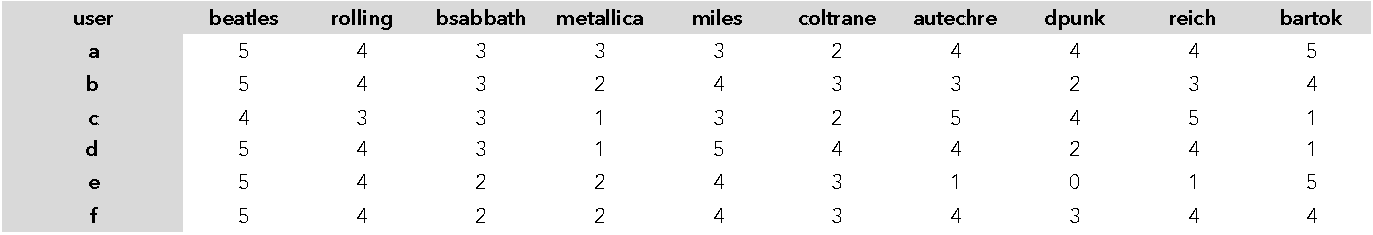
\includegraphics[width = 1.0\textwidth]{six_users_factorization_machines_4.pdf}
% \caption{Estimated preference values for all users of synthetic example}
% \label{fig:six_users_factorization_machines_4}
% \end{figure}

% From the previous synthetic example it can be seen how it is possible to incorporate side data features using the factorization machine technique in order to preference of users on items. The factorization machine model thus extends the classic model of matrix factorization by including in the model all pairwise interactions of side features variables to the user and item data. 
% \textcite{rendle11fast} described how this technique could be used to model contextual information and provide context-aware rating predictions.
% \textcite{rendle13scaling} applied this approach to the Netflix prize dataset, incorporating side features to reducing the RMSE in predicting the number of stars a user assigns to a movie. 
% The results of the experiment showed that incorporating more side features into the model, such as day of the week of rating, and a list of all movie IDs a user ever rated, dropped the error largely. The author also tested the model in the KDDCup2012 dataset, which task is to predict which tweets a user will follow. Again, side features such as reported age and gender of users, tweet keywords, number of tweets, and the list of friends of the users were incorporated in order to improve the precision of the model. 
% The results of both experiments showed that the factorization machines model effectively is able to incorporate contextual information of users and items for the reduction of error and improvement of precision. In both cases, however, the extra information was not enough to reach the values of the winning approaches, finishing with a RMSE value of 0.88 in the Netflix Prize dataset, and within the Top 5 in the KDDCup2012 leaderboard.























% %--------------------------------------------------------------------
% % CF CHALLENGES
% %--------------------------------------------------------------------

% \subsection{Collaborative filtering characteristics and challenges}

% CF algorithms have limitations and challenges that have to be addressed in order to create better recommendation systems. As CF relies on explicit ratings of users on items, or implicit preferences of listeners on songs, the more preferences an item has, the more accurate the recommendation system is. Furthermore, when preference data is sparse, the quality of the recommendation is less reliable. Moreover, as users in real-life applications usually have not accessed all items in a recommender database, not all items in the database have rates and so they will be hardly recommended \autocite{breese98empirical}. In the context of online digital music services this is evident. It is unlikely that a song that just entered the system database be accessed and rated by any listener, and so a recommendation for it will be improbable until enough preferences for this song have be established. An analogue drawback can be seen for listeners that just join a music recommender system. It is probable that the quality of the recommendation will be poor because they have provide the system with none or just a few ratings, and so their listening profile is still limited. Also, as noted by \textcite{song12survey}, because of the subjectivity in music, the premise that users with similar behaviours may have alike tastes has not been widely studied. Furthermore, how best to measure user similarity and assess its unpredictability? Also, how to aggregate divergent opinions from various users? Finally, should all data be trusted equally or can one detect or intentionally misleading opinions? 

% % \shortciteANP{su09survey} (2009) notes that some model-based CF systems have downsides, such as expensive processing procedures when learning the model, decrease in performance when doing dimensionality reduction, and impractical when data is extremely sparse because the model is hard to create accurately. However, these problems, or related ones, also appear in memory-based systems.

% The next list formalizes the problems just expressed, and reviews other characteristics and challenges that CF methods of any domain, not only in music, have.

% \begin{description}
% \item[Data sparsity] 
% In large databases, the user-item matrix can be very large. The data can become sparse, and the performance of the recommendation can be challenged. The problem of data sparsity appears in many forms affecting the performance of the system and the quality of the recommendation. Among these forms, the most the \emph{cold start} problem, the \emph{reduced coverage} problem, and \emph{neighbour transitivity} are the most common ones.

% \item[Cold start] 
% One typical CF problem is the \emph{cold start} or ``startup problem''. When a new user, or item, has just entered a database, it is difficult for the system to find similar ones because there is not enough data to find a neighbour. Thus, new items cannot be processed properly until some users rate it, but also new users will not receive good recommendations because of their lacking of rating or behavioural history \autocite{herlocker04evaluating}.

% \item[Coverage] 
% Coverage is the proportion of items that the system can provide recommendations for. The reduced coverage problem appears when the number of users' ratings is very small in comparison with the number of items in the system, and so the algorithm cannot generate recommendations for many of them \autocite{herlocker04evaluating}.

% \item[Neighbour transitivity] 
% The neighbour transitivity problem appears in sparse databases where users with similar tastes cannot be recognized as similar because they have not rated the same items. Thus, a system relying on comparing users in pairs cannot generate predictions if there is not enough ratings \autocite{su09survey}.

% \item[Scalability] 
% When the number of users and items becomes large, traditional CF methods suffer of scalability problems. For example, with 10MM users ($M$) and 1MM items ($N$), a CF algorithm will have a complexity of at least $\mathcal{O}({M}\cdot{N})$. Also, recommendation systems usually have to react instantly to online users' requirements, as well as incorporate fast in the system the addition of new items as well as new users. As the computation of all distances can not be done every time a new item or user is added, several techniques have been developed to handle this problem, such as the dimensionality reduction singular valued decomposition CF algorithm, the Pearson correlation CF algorithm, and clustering CF algorithms \autocite{su09survey}.

% \item[Synonymy] 
% Synonymy refers to the propensity of items to have several versions of its name or attributes. In other words, the same item might have been labelled in different ways, and so the system treats them as different entries. For example, the artist Michael Jackson can appear in the same database as Jackson, Michael; M. Jackson; or M. Jacson. As the synonymy problem decreases the performance of CF recommendation systems, during the stage of preprocessing of entries in the database, the several version names are normalized, usually by using edit distance, term expansion, or by building a thesaurus \autocite{su09survey}. 
% A related problem to synonymy is polysemy, which refers to several meanings of the same item \autocite{levy08learning}. This problem is common in web queries, but less common in the context of music where artists try to find unique names for their songs, album names, and themselves. However, a simple search for the artist name ``Sugar" in Musicbrainz\footnote{\url{http://www.musicbrainz.org}} retrieves eight entries for this band's name: a Korean group, two Japanese groups, an afrobeat group, the alias of an Australian producer, an alternative rock band, a dance group, and a Puerto Rican religious artist. In the case of the Musicbrainz database, they have implemented a disambiguation field to try to discriminate the several entries.

% \item[Gray and black sheep] 
% Gray sheep refers to users whose preferences do not consistently agree or disagree with other users, and thus they do not benefit from CF. Black sheep are those users with very peculiar preferences, and so the system can not make recommendations for them. This last problem also appears in non-automatic recommender systems, and so it is considered as an acceptable failure~\autocite{su09survey}. 

% \item[Shilling attacks] 
% The shilling attacks problem appears when the rating of some users on items is biased to a subset of them. For example, by giving very positive rating on their own material, and very poor on their competitors. In other words, malicious users are logged in the system to to push predictions of some targeted items~\autocite{su09survey}.

% \item[Personal privacy]
% CF-based recommender systems have also posed interesting problems about personal privacy because they rely on the preference and habits of people. However, people may not want their habits or preference be widely know. Because of this, recommender systems usually allow anonymous participation under a pseudonym. However, research by \textcite{narayanan06robust} showed how users in large datasets can be de-anonymised, uncovering potentially sensitive information.

% \item[Other characteristics] 
% The idea of \emph{explainability} has been proposed by \textcite{ross08recommendations} to express a beneficial concept that might be exploited for recommendation systems. Explainability adds a dimension of ``reasoning" to the recommendation engine, for example, by telling the user ``you will like this song because you previously liked songs \emph{A} and \emph{B}''. Thus, the user can be able to understand why the system recommended a specific item to her, thus integrating the user into the recommendation ``black-box" process. In other words, instead of just having a list of songs, the listener might benefit of knowing why those songs were recommended. Explainability might also be used to introduce new items to users, for example, to recommend new released songs or new artists, thus helping to overcome the cold start problem.
% \end{description}



















% \subsection{User tasks for recommender systems}
% \textcite{herlocker04evaluating} state that the evaluation process of a system should begin by understanding the user tasks that the system will serve. Hence, they investigated and described the most significant tasks performed by people when using recommendation systems, which are described in the following list.

% % \newline

% \begin{description}
% 	\item[Annotation in context] The user wants to distinguish desired and undesired content, thus recommender systems help to annotate, tag, or filter items.
% 	\item[Find good items] The user wants to find some items for some specific reason, and the recommender system provides a commonly ranked list of suggestions.
% 	\item[Find all good items] In contrast to finding a good recommendation, sometimes, a user wants to find all items related to a specific query.
% 	\item[Recommend sequence] Instead of looking for one item at a time, the user is looking for a sequence of items that are pleasing as a whole.
% 	\item[Just browsing] The users use this approach when they just want to spend time browsing the system by pure pleasure.
% 	\item[Find credible recommender] People use this approach when they want to ``play around'' or test how the recommender system works or matches their tastes. 
% \end{description}

% Each of these tasks has different characteristics and attributes, and so for evaluating a recommendation system from the perspective of the user task, a specific metric or set of metrics, and an experimental setting, have to be considered.







% %  \shortcite{lu12recommender}


% Comprehensive evaluations of recommendation systems do not use just one approach, because each one addresses different properties and characteristics of the system. Also, the overall user experience with a given recommendation system---which includes the user satisfaction with the recommendation---is difficult to measure in ``offline'' evaluation, and so empirical user studies represent a welcome source of feedback on recommender systems. Consequently, an extensive offline evaluation is typically run first to discard some of the algorithms; then, a user study allows to measure the reaction of user on a subset of systems; finally, a online evaluation is performed to measure directly the overall goals of the system. 

% The next section provides an overview of recommendation system properties and the metrics usually used to measure them.

% \subsection{Evaluation metrics}

% So far, we have seen that most commercial recommender systems use the opinions of a community of users in order to help other users in that community to find content of interest in a potentially overwhelming set of choices. However, there are many approaches and algorithms available for generating recommendations, each of them with unique characteristics and attributes that define their specific behaviour. Identifying the best approach to fulfil a specific information and recommendation need has to consider the characteristics, strengths, and weaknesses of each method and domain.

% The evaluation and comparison of recommendation systems is particularly difficult. First, the goal of users when using various systems can be different, and so the approach and properties to evaluate them should be different too. 
% Second, some algorithms perform better on some datasets and worse on others, and so a proper comparison should have same or similar data. 
% Finally, a single metric cannot be used to decide the best algorithm because it will measure a single aspect of it, and therefore a combination of metrics will provide a broader point of view when doing a comparative evaluation. 
% Consequently, there is also a challenge to decide what combination of metrics to use \autocite{shani11evaluating}.




\section{Recommendation system evaluation}\label{sec:ch4-evaluation}
Evaluation of recommendation system properties is complex. 
On the one hand, the systems can have different goals and so some of the properties that describe them can be more, or less, linked to those goals. Therefore, the metrics to use when evaluating recommendation systems should be the ones that are linked to the properties related to those goals. Otherwise, there is potential for an inaccurate measurement of tasks. 
On the other hand, there is a lack of standardization of evaluation metrics, and so it is common that researchers introduce new metrics when evaluating their systems, which makes it hard to compare results among systems. 
In spite of that, we will now present the most standard evaluation metrics for recommendation system, consolidated from a number of studies \autocite{goldberg01eigentaste, herlocker04evaluating, su09survey, celma10music, shani11evaluating, lu12recommender}. 
Broadly speaking, there are two sets of metrics: accuracy metrics and usefulness metrics.

\subsection{Accuracy metrics}
Accuracy metrics measure how well a recommender system can predict an exact rating or preference value for a specific item, or how close a predicted ranking of items for a specific user is to the user's true ranking of preferences. 
Depending on the recommender goals, accuracy metrics can be used to measure prediction, classification, or ranking.
	
	\begin{description}
		\item [Predictive accuracy metrics] are used when we want to predict the rating, or preference, a user would give to an item. This metric is computed by comparing the predicted rating on an item with the actual value a user has expressed about it. 
        
Root mean squared error (RMSE) is the most commonly used metric for evaluating accuracy of predicted ratings. RMSE is formalised as:
		\begin{equation}\label{eq:rmse} 
			RMSE= \sqrt[]{\frac{1}{|\mathcal{K}|}\displaystyle\sum_{(u,i) \in \mathcal{K}}(\hat{r}_{ui} - r_{ui})^2}
		\end{equation}

		where $\mathcal{K}$ is the given test set of all user-item interaction pairs $(u,i)$, $\hat{r}_{ui}$ is the predicted rating calculated by the recommender, and $r_{ui}$ is the rating value actually given by the user on the item. 
        
Mean absolute error (MAE) is an alternative to RMSE that penalises large errors to a lesser degree:
		\begin{equation}\label{eq:mae} 
			MAE = \frac{1}{|\mathcal{K}|}\displaystyle\sum_{(u,i) \in \mathcal{K}}|\hat{r}_{ui} - r_{ui}|
		\end{equation}

Derived from these metrics, researchers have developed several related metrics, such as Average RMSE, Average MAE, Normalised RMSE, and Normalised MAE. These alternative metrics aim to compensate for errors coming from datasets with an unbalanced distribution of items, or for ranking scales that are not fully used.

Predictive accuracy metrics have benefits such as easy implementation and computation, and are also conceptually easy to understand. These advantages make them a commonly used set of metrics to compare the predictive accuracy between recommender systems. 


		\item [Classification accuracy metrics] measure the frequency with which a recommendation system makes good decisions about ``whether an item is good or not". These metrics are usually used for tasks of finding relevant items, where the recommendation engine does not try to predict the user's preference or rating on items, but to recommend items to users that they may use or like. In this case, the possible outcomes of the recommendation belong to two classes: relevant or irrelevant items. These classes are organised into the following categories:

		\begin{description}
			\item True positive (TP) for recommended items the user is interested in.
			\item False positive (FP) for recommended items the user is not interested in.
			\item True negative (TN) for not recommended items the user is not interested in.
			\item False negative (FN) for not recommended items the user is  interested in.
		\end{description}

		Based on these four possible outcomes, two commonly used classification metrics are defined: precision and recall.

		\begin{description}
			\item \emph{Precision} measures the fraction of relevant retrieved items over all the recommended ones. It represents the probability that a selected item is relevant. Precision is formalised as:
			\begin{equation}\label{precision} 
			% \vspace{1em}
			Precision = \frac{TP}{TP + FP}
			\end{equation}


			\item \emph{Recall} measures the fraction of relevant instances that are retrieved. It represents the probability that a relevant item will be selected. It is formalised as:
			\begin{equation}\label{recall} 
			Recall = \frac{TP}{TP + FN}
			\end{equation}
		\end{description}

If the user does not need a full list of potentially relevant items, for example when using the recommendation system to find a good item, precision alone at a single search length or a single recall level can be appropriate. However, if the task implies finding all good items, recall becomes important. 

Precision and recall are inversely related and depend upon the length of the result list returned to the user. If a higher recall is allowed, it is likely that precision will be lower. If recall is low, the precision is usually high. Because of this trade-off, it is common to use a single metric to express both precision and recall with a single number. This metric is known as the F-score.
F-score combines precision and recall into a single value. Their respective importance is weighted by adjusting a $\beta$ factor. A value of 1 for $\beta$ implies same weight for both precision and recall, in what is known as F\textsubscript{1} score or F-measure. The F-score is formalised as:
		\begin{equation}\label{fscore} 
		F_\beta = \frac{(1 + \beta^2) \cdot (Precision \cdot Recall)}
					{\beta^2 \cdot (Precision + Recall)}
		\end{equation}

% 	An alternative to using precision and recall, is using \emph{ROC curves}.

% 	\begin{description}
% 		\item \emph{Receiver operating characteristics curves} (ROC)  illustrate the performance of a binary classifier as its discrimination threshold is varied. 
% 		It is a plot of the true positive rate (i.e., sensitivity, the fraction of TP out of the positives, or the percentage of good items returned) in function of the false positive rate (i.e., 100-specificity, the fraction of FP out of the negatives, or the percentage of bad items returned), at various threshold settings. Therefore, it shows the trade-off between sensitivity and specificity of the classifier for all threshold values. 
% 	\end{description}
	
% %     Explain for my own research
    
% 	The area underneath a ROC curve (AUC) provides a single number to discriminate between good and bad items, and represents the overall classification accuracy performance of the system over all different recommendation list lengths. ROC Curves are used to see how well the classifier can separate positive and negative examples and to identify the best threshold for separating them. Possible AUC values vary between 0.5 (pure chance) and 1.0 (perfect classification). %check http://mlwiki.org/index.php/ROC_Analysis for explanation and how to select best threshold

% 	Depending on the goal of the application, precision-recall and ROC curves might be used to measure classification accuracy. Precision, for example, would be useful to describe if the proportion of recommendations produced by a recommender was suitable for a user. ROC curves, on the other hand, might be helpful if we want to choose a large set of items to making recommendations to users with no penalty if they do not like them.

All in all, precision, recall, and F-score are well tailored to binary retrieval contexts, where recommended items can be categorised as relevant or irrelevant, but their ranking is not important. 
If the ranking of the retrieved relevant items is important, rank accuracy metrics can be used.
\end{description}

\begin{description}
	\item [Rank accuracy metrics] are used when we want to measure how much an ordered list of items given by a recommender matches how a user would have ordered the same list. Hence, these ranked-based metrics are not usually used to just find relevant items because they can be over-sensitive for this task. 
There are several approaches for evaluating a ranked list of recommendations, but basically they are based on the correlation of lists of items or in their utility. 
While the former approach compares a ranked list of recommendations with a reference ranking, the latter measures the utility of the predicted list, assuming that top positions in the list are more relevant for the user than the ones in the bottom of the list.
\end{description}

So far, we have reviewed evaluation metrics only based on intrinsic properties of the recommendation system. However, system-centric evaluation has some limitations. 
First, users usually do not rate all items in the recommendation system database, and so the observations that a system-centric approach can evaluate is a narrow, probably biased, subset of the total number of items. 
Second, the \emph{perceived quality} of the recommendations cannot be measured because system-centric evaluation does not pay attention to user satisfaction or to the perceived quality of the recommendation \autocite{adomavicius05toward}. 
In short, automated recommendation systems can be evaluated not only by accuracy metrics, but also by their \emph{usefulness}.






\subsubsection{Beyond accuracy: Usefulness} \label{section:usefulness}
Current recommendation systems should also satisfy users in terms of the appropriateness and perceived quality of the recommendation. The user's perception is multidimensional by nature, and so several measures have been proposed in the literature to describe and evaluate recommender system properties from a user-centred point of view \autocite{herlocker04evaluating, celma08new, shani11evaluating, knijnenburg12explaining}. 
These properties, and pertinent metrics if any, are explained below.

% Some of these properties are coverage, novelty and serendipity, confidence and trust, diversity, learning rate, utility, and robustness.  

\begin{description}
	
	\item [Coverage] is a measure of the domain of items for which the system can generate predictions or recommendations. The most common metrics for coverage are the ratio of items for which predictions can be generated and the total number of items, and the ratio of items for which predictions can be generated and the total number of items in which a user \emph{may have interest}. Coverage is usually linked with accuracy in order to not raise coverage by making dummy predictions for every item.  
	
	\item [Novelty and serendipity] are properties for generating useful and meaningful recommendations. Even if recommendations are accurate and have high coverage, they can be bogus if the user expects some surprise and freshness. While serendipity refers to the quality of finding surprisingly interesting items that the user might not have otherwise discovered, novelty refers to the discovery of new items. Hence, serendipitous recommendations are by definition novel; the opposite is not necessarily true. 
	% 	An interesting fact about measuring serendipity is that, by definition, it relies on the opposite of measuring accuracy, which uses past preferences as indicators for recommending new items. 

	As observed by \textcite{herlocker04evaluating}, developing metrics for novelty and serendipity is still an open problem, but they should look at how well the recommendation system makes the user aware of previously unknown items. Furthermore, serendipity metrics should also consider how the interests of users change over time.
	However, it seems that novelty and serendipity are user-specific parameters. \textcite{zhang12auralist} performed a user-centric evaluation of a music recommendation framework with a series of algorithms that improved its diversity and novelty with a trade-off in accuracy. The authors found that the majority of people favoured greater accuracy, however some people accepted a loss of accuracy as a trade-off for greater serendipity. 

	\item [Diversity] is a recommendation property that assumes users want to explore the range of items instead of only being recommended with similar, accurate ones. Although diversity has a trade-off with accuracy, people value obtaining more diverse recommendations. 
%     Diversity is usually measured by using item-to-item similarity. %example: reporting range of hotels for a vacation package, not the same type

	\item [Confidence and trust] are complementary properties related to credibility. While confidence can be seen as how sure the system is about the recommendation it provides to the user, trust refers to how much the user relies in the system's recommendation. Hence, trust is built upon the interaction between system and user. While a common metric for confidence is the probability that the predicted value is indeed true, there is no clear metric for measuring trust. As a consequence, trust is usually measured by asking people in user studies, or derived from user behaviour in online experiments. Reporting confidence scores may also be beneficial to enhance the user's trust in the recommender \autocite{herlocker00explaining}. 

	\item [Learning rate] is an important property of recommender systems because the recommendation quality depends upon the quantity of data. For example, if there is not much initial rating data we may have a ``cold-start'' problem. Also, if there is not much data in the form of implicit or explicit preferences provided by users, the system may not be able to provide any useful recommendations. Although there is usually a lack of evaluation of this property, the amount of data needed to provide meaningful recommendations might be seen as a logic metric.

	\item [Utility] is the value that the user, or system, gains from the recommendation. Utility can be considered more significant than just measuring the accuracy, coverage, or other properties of the recommendation, but it can be harder to measure. In e-commerce contexts, utility is usually linked to the revenues provided by the recommendation engine, and so online retail websites try to improve their revenues by testing new or variants of their recommendation algorithms on some users, and analyse their purchase behaviour.
	
% 	\item [Robustness] refers to how stable the recommendation system remains in the presence of fake information or \emph{shilling attacks}, or how stable it is under extreme conditions such as a large number of requests.

	% \item [Adaptivity]
	% \item [Scalability]
	% \item [User evaluation]

\end{description}







% Extensive research has been done for evaluating recommendation algorithms, however the lack of standardized datasets and metrics have made it difficult to compare different approaches. The next section, however, will review some of the most common datasets that have been used to evaluate general recommendation systems. 




% \subsection{Evaluation datasets} \label{section:datasets}

% There are several open-source datasets with real data that have been used to measure and compare the performance of individual recommendation algorithms. As these are datasets for offline evaluation, only accuracy and ranking metrics are typically computed and compared. We now provide a review of some of these datasets in the domains of movies.

% \begin{description}
% 	\item[Movielens dataset] Movielens is a virtual community and movie recommender system. Since 1997, they have collected user ratings on movies and have released datasets for the evaluation of CF algorithms.\footnote{\url{http://www.grouplens.org/node/73}} The data they provide forms a 4-tuple in the form: (\emph{UserID}, \emph{MovieID}, \emph{Rating}, \emph{Timestamp}), where ratings are made on a 5-star scale and each user has at least 20 ratings. Currently there are three datasets available: MovieLens 100k, MovieLens1M, MovieLens 10M, according to the number of recorded ratings. 
% 	This dataset has more users than movies, and so is especially well formed for such cases.


% % MENTIONED BEFORE
% 	\item[Netflix Prize] The movie subscription rental service \emph{Netflix} released in 2006 a dataset containing roughly 100M time-stamped ratings from 500K anonymous subscribers, on nearly 18K movie titles. The data reflected the distribution of all ratings (in a discrete scale) received by Netflix during a 7-year period. The whole dataset was divided into subsets for training, validation, and testing (96, 1.3, and 2.7 percent of the whole dataset respectively). 
%     Netflix challenged the research community to develop a recommender system capable of improving their own movie recommendation system on at least 10 percent, and offered a prize of one million dollar for the winner. Netflix's own recommendation system tried to predict the number of stars that a person would rate a video after watching it, on a scale from 1 to 5.
%     The improvement in accuracy should be computed using the RMSE of the system's prediction against the actual rating that a subscriber provides. 
%  \autocite{bennet07netflix}. 

% 	The big lesson from the Netflix competition come from the fact that there was not a unique algorithm that achieved the desired accuracy improvement, but teams had to join forces--- and algorithms---in order to reach the mark. Thus, after three years of work, the top two teams beat the challenge by combining other teams' ideas and algorithms into more complex algorithms. Different teams had different approaches, and, when combining them, the accuracy got better.\footnote{See the leaderboard of teams and their marks at \url{http://www.netflixprize.com//leaderboard}} For example, ``BigChaos'', one team of the winning team, devised a three-dimensional model that incorporated time into the relationship between people and movies. Thus, the winning teams developed hundreds of predictors and used an iterative process where the predictor with the lowest contribution was removed. In the end, 18 predictors were used to achieve 10 percent improvement \autocite{toscher09bigchaos}.


% \end{description}




\subsection{Experimental settings}\label{sec:experimental_settings}
Typically, there are three main experimental settings to test and compare general recommendation systems, regardless of their domain \autocite{herlocker04evaluating, shani11evaluating, lu12recommender}.

\begin{description}
	\item[Offline experiments] This approach is typically used when there is pre-collected data of user preferences. It assumes that future behaviour of users will be similar to user behaviour when the data was gathered. An offline experiment requires no interaction with real users and so it is usually easy and fast to implement, permitting comparison of several algorithms at low cost. 
    The main downsides of this approach are: it only provides results for a specific set of predictive accuracy metrics, does not measure the user behaviour change over time, and cannot express the overall user satisfaction and experience. In spite of these limitations, offline experiments have been the most used experimental settings for the evaluation of recommendation algorithms and systems. 
	
	\item[User studies] In this approach, subjects are instructed to perform a set of tasks while interacting with a recommender system. Behavioural features are collected over time, and qualitative questions are asked before, during, and after the task is completed. These qualitative questions usually help to understand quantitative data and data not directly observable, such as interface enjoyment, or overall user perception about the system. Limitations of user studies are their cost and possible biases in the sample of the population. 

	\item[Online evaluations] These tests measure the behavioural change of real users when using recommendation systems. This is accomplished by redirecting a portion of the traffic of users to different recommendation engines, and recording the users interaction with the different systems. In a sense, this setting provides the strongest evidence of the true value that the user perceives from the system. Typical factors to take into account when implementing online experiments are to obtain a properly sampled population of users and to isolate the variables that are going to be tested. 
\end{description}



Recommendation evaluation is a multi-dimensional problem, with many features that are measured in parallel. Hence, the ultimate validation is performed in real-life, when the systems have been deployed, enough interaction data has been collected, and people have integrated them in their behaviour. Then, the perceived quality of the recommendations may be evaluated indirectly by measuring how much people use the systems over time, by quantifying the length of listening sessions or, ultimately, by looking at the increase or decrease of global number of users of the system \autocite{gomez15netflix}.


\section{Music consumption uniqueness}
Although the same recommendation frameworks are typically used for recommending books, movies, restaurants, or electronic products, music and music consumption are inherently different than other types of media and consumer goods. % STRAW 2
The large variability in users' tastes in music and their music consumption behaviour present challenges that are different from other domains. As a result, it may be beneficial to consider the special nature of music when building automated music recommendation systems in order to provide a better, more enjoyable experience.

We now present a compilation of the features of music consumption that have been stressed as distinctive in comparison with other domains in studies by \textcite{denora00music, north04uses, casey08content, jones08user, park10temporal, celma10music, baur11thesis, celma11tutorial, song12survey, zhang13understanding, margulis13onrepeat}.


\begin{description}

	\item [Huge item space] Music is nowadays easily available in massive repositories. Compared to other domains, the space of recommended music items is fairly large. For example, typical online music stores and digital music services currently offer 30 million titles to choose from. 
	% As pointed out by \textcite{lacher89hedonic}, it is worth noting that music is initially consumed through diverse media vehicles before a user actually buys a music item. And so, currently the largest music delivery channel is the video-sharing website YouTube, which provide access to even larger quantities of musical items.
	Also, advances in technology such as storage format, Internet access, and device portability have resulted in changes in the abundance, ubiquity, and in the way people interact with music. Modern portable devices allow people to access million of songs wherever they go. These devices also make it possible to listen to music in many diverse listening contexts in a person's day-to-day life.

	\item [Item formats] Music these days is accessible in a wide range of formats and varieties. In addition to classic physical formats, non-physical digital delivery of music is a common format for buying music. However, music is also enjoyed by streaming it from online repositories. Video-sharing websites such as YouTube provide access to a large variety of music item types, such as songs, full albums, concerts, remixes, documentaries, or video-clips. 

	\item [Low cost per item] The perceived cost per song in music streaming services is negligible. This implies that music listening has very small financial commitment compared to other entertainment-related commodities. Although this characteristic allows people to access music easily and painlessly, it also poses a challenge in the sense that music is nowadays so easy to acquire, that it is seen as a commodity. Most listeners are unlikely to spend much money choosing specific music items, they just stream songs, but do not ``treasure'' them. 
	
	\item [High reuse per item] Unlike the consumption of movies, books, or games, people listen to recorded music more than once, in different moments and contexts. People enjoy listening to music repeatedly and continuously.

	\item [Consumed in sequences] People enjoy listening to sequences of songs, often getting as much enjoyment from the song transitions as from the songs themselves. Hence, listening to music is not a process of enjoying isolated music items one after another, the whole listening session is important. 
	It is also common that if a song does not fit the listener's mood, the person may skip songs until the proper one fits what the listener wants to achieve.

	\item [Highly contextual usage] As listeners have different  preferences for music based upon their context and activities, the listening context seems to influence the value of the music item and of the musical experience to the individual listener. For example, a playlist for physical training is likely to be different than a playlist created by the same person for relaxing or having dinner.

	\item [Low attentional demand] Unlike watching videos or reading a book, listening to music does not require one's full attention. Also, people are commonly engaged in other activities while listening to music. Many times the focus of attention is not on the music, but instead it is used as a background to other activities, or to reconstruct the aims of those activities. 

	% \item [Highly social] Some authors have noted that music listening is a highly social activity \autocite{celma10music,celma11tutorial}, but others have indicated that the liking for music heard in isolation is higher than liking for music heard in the presence of others\autocite{north04uses}.

	\item [Low consumption time] People interact with music in a different way than they do with other types of media, such as books or movies. One reason for this is because music items such as songs or albums usually have a shorter consumption duration. For example, a new song can be heard in matter of minutes, whereas a movie may be watched in a couple of hours, and a book may be read in a few days. 
	For music recommendation, this feature implies that a shorter validation process is needed to determine the quality of the recommendation. In other words, listeners can more quickly and easily determine if a recommended song is enjoyable, in comparison to recommendations from other domains

	\item [Portability] In combination with music streaming services, smartphones can be used as music media players anywhere, anytime, without the need of any other device, and so music can be consumed anywhere. This is different to video streaming, for example, which requires special conditions of light and screen size, at the least.

\end{description}

In this chapter we reviewed how the recommendation problem is formalised, the different approaches for implementing automated recommendation systems, and summarised the metrics and the experimental settings for the evaluation of these systems.
In the next chapter we will provide details about the creation of a large dataset of music listening histories with the ultimate goal of evaluating if user-centric features extracted from these listening histories can improve the accuracy of a music artist recommendation model.
We will describe the criteria for the data collection, preprocessing, and aggregation. Then we will summarise the characteristics of the dataset as well as the demographic features of listeners, and we will finalise the chapter by presenting how we were able to time-align the music listening histories from more than half-a-million listeners from more than 200 different countries.






% % \section{Issues}\label{sec:issues}









% \section{Context and recommender systems}\label{sec:4-context-and-recommender-systems}

% As reviewed in previous sections, extensive research has been done on recommendation systems in the past decades. However, recommendation techniques still cannot completely understand, or predict, the users' information needs while searching for items. In fact, the ephemerality of the need, but also the context of the search and of the item's usage, do influence users' perceptual evaluation of the recommendation \autocite{ricci12contextualizing}.
% In addition, previous findings in behavioural research suggested that decision making is not invariant, but is dependent on context \autocite{klein89context, bettman91consumer}. 
% As a consequence, the context of the interaction should be taken into account when generating recommendations that users would judge as appropriate to their situations. 

% In this section we provide an overview on the concept of context in the interaction between human and computers. We also formalise an approach to incorporate contextual dimensions in the recommendation process, and present previous research on recommender systems that have implemented contextual dimensions as part of their input data and processing.


% \subsection{Understanding context in human-computer interaction}

% When people interact with people, they make use of implicit situational information---\emph{context}---in order to increase their conversational bandwidth \autocite{abowd99towards}. However, in traditional interaction between human and computers, this ability of transferring underlying ideas is much less feasible. 
% As a consequence, finding ways to improve the access of computers to the constantly changing context of users---due to hand-held and ubiquitous computing everywhere---should enrich the human-computer communicational interchange, making computers to produce more useful and tailored recommendations \autocite{herlocker01content}.

% Various definitions of context have been proposed in the literature over the years.
% \textcite{schilit94disseminating} defined context as the location, the collection of nearby people and objects, as well as the changes to those objects over time. They also coined the term \emph{context-awareness} to describe software with the capability of changing its behaviour according to user's contextual features. 
% \textcite{brown97context} proposed adding time, temperature, and season to characterize the context of people, on top of the characteristics proposed by \textcite{schilit94disseminating}.
% \textcite{ryan98enhanced} suggested that location, environment, identity, and time were also important elements in defining context.
% \textcite{franklin98gadget} stressed the concept of environment, stating that context is the user's environment.
% \textcite{dey01understanding} defined context as the whole situation relevant to a user and an application. He emphasizes, however, that it is not possible to enumerate a specific, unique set of attributes common to all circumstances because the importance of these characteristics changes for every situation. 
% Hence, \textcite{dey01understanding} prefers to re-define context as any \emph{relevant} piece of information that can be used to characterize the situation of a participant in the interaction with a computing application. According to his definition, there are elements that are part of the context in some situations, but are not in other circumstances. He extrapolates this idea to context-aware systems, stating that a system is context-aware if it uses contextual information to provide relevant services to the users, where relevancy is dependent on the user's tasks.
% %e.g., weather can be important for outdoor, but not for an indoor mobile tour

% Conventional recommender systems usually only make use of previous users' preferences, similarities between items or between users, or a combination of these, to make recommendations. 
% However, users' preferences change according to their context, and so their specific contexts have to be considered in order to improve the perceived quality of the recommendation. The next section formalizes an approach for incorporating the contextual dimension in the process of recommendation.

% % The use of contextual features has not been extensively used in recommendation system yet, however the next section presents previous research about their use in recommendation systems of various domains. 

% %baur11thesis: Lifelogging concept

% \subsection{Incorporating context in the recommendation process}

% We have seen in previous sections that conventional recommendation approaches make use of a two-dimensional paradigm of $Users\times Items$ . For incorporating context to this model, \textcite{adomavicius01multidimensional} proposed a \emph{multidimensional recommendation model} that can generate recommendations based on multiple dimensions.
% In their approach, the \emph{recommendation space} is given by dimensions $D_1, D_2, ... ,D_n$ where, instead of storing the preferences of users on items in a two-dimensional matrix, a multi-dimensional matrix is used. Hence,  the \emph{rating} or \emph{preference function} is defined over the space $D_1\times D_2\times ...\times D_n$. 
% % In their approach, the \emph{recommendation space} is given by dimensions $D_1, D_2, ...\hspace{2px} ,D_n$ where, instead of storing the preferences of users on items in a two-dimensional matrix, a multi-dimensional matrix is used. Hence,  the \emph{rating} or \emph{preference function} is defined over the space $D_1\times D_2\times ...\times D_n$. 
% To exemplify this, we might consider a three-dimensional recommendation space of $Users\times Songs\times Time$, where each dimension is defined by a set of attributes that create a profile, such as $User\subseteq UserName\times Address\times Gender\times Age$, $Song\subseteq SongName\times Artist\times Album$, $Time\subseteq Year\times Month\times Day\times Hour$. In this multi-dimensional space, implicit preferences of listeners on songs can be stored, but these preferences are also related to a temporal factor.
% The profiles for each dimension can also include information extracted directly from the data, such as statistical attributes, rules describing relations between elements in the database, or sets of behavioural sequences. 
% In \textcite{adomavicius05incorporating}, the authors also formalized and implemented a \emph{reduction-based approach} in their multi-dimensional recommender that involved using ratings only related to the current context of the user to make recommendations, and so the multi-dimensional recommendation space was reduced back to the $Users\times Item$ space. 

% Hence, a multi-dimensional recommender system can expand the possibilities of recommendations, such as offering ``best $N$ user/time combinations for each song,'' or ``best $N$ songs to recommend for each user/time combination,'' or ``best $N$ times to recommend for each user/song combination,'' or any other possible combination. 
% Furthermore, as we have seen on chapter~\ref{ch:2-human-music-listening-interaction}, there are other music listening context features that affect our perception about music such as \emph{activity}, \emph{companion}, and \emph{place}, and so including these in a multi-dimensional recommender scheme might be sensible. 
% As a consequence, a multi-dimensional recommender system would be able to express not only preferences on songs by listeners, but also correlate those with where the listening experience is happening, what activity the listener is doing, and with whom listeners are. \textcite{stober09survey} went even further and also proposed to include \emph{GPS position}, \emph{ambient noise}, \emph{ambient light} and \emph{bio-information} as features to express listening context. 
% However, these latest suggestions rise the question of what dimensions really matter and which dimensions could be safely dropped for creating efficient multi-dimensional models of recommendation.
% Moreover, it is also unclear at to what extent the additional charge placed on the user will result in a reduction in usage of the recommendation system. This question is based on the fact that the user has to provide more data to the system, and this process might not be seen central to the task at hand, or might rise concerns about privacy \autocite{anand07contextual}.

% % In MD recommendation spaces, processes of feature selection are usually performed to obtaining a minimal subset of features so that the original task can be achieved equally well in a reduced set. If properly chosen dimensions are discarded, a reduced MD space might offer a better representation of the whole data population \shortcite{liu98feature}. 







% \subsection{Use of context in recommender systems}
% %Provide a detailed literature review in recommender systems that have investigated and implemented any kind of contextual dimensions.

% As expressed previously, user's preferences change according to the user context. Hence, the recommendation offered by a recommender system considering user's context should be better. We now provide a review of research on recommender systems that have implemented any kind of contextual dimensions as part of their input features.

% % restaurants
% \textcite{pazzani99framework} used users' demographic data such gender, age, and area code, to create users' profiles and to relate single items to groups of people that like that object, based on their demographic data. He implemented a hybrid approach that combined five collaborative-filtering, content-based, and demographic-based recommendation algorithms to generate better restaurant recommendations.
% % movies
% \textcite{ansari00internet} also used contextual information of individual demographic characteristics, such as age and sex, but they combined these features with item's characteristics, user's explicit and implicit preferences, and expert's judgements on items, to predict ratings on movies. Their recommendation method achieved better performance than classic recommendation approaches that did not consider user profiles.






% % music
% \textcite{hu11nextone} created a system that recommended songs based on user behaviour. Their approach considered gender, recording year, and time patterns as factors to recommend songs. They based the evaluation of their system on collecting user's listening logs and skipped songs, calculating the number of songs played per day and the running time of each listening session. Their results showed an increase in the number of songs listened to per day, and a decrease in the number of skipped songs.
% % music
% \textcite{hayes04context} captured listeners' context by using content-based analysis techniques on song playlists. They hypothesized that context is a content-based representation of items currently being experienced, and that human-created playlists capture some implicit rules when putting together selections of songs. Hence, some aspects of the ``task context'' could be extracted from the analysis of those playlists, and these can be used to refine recommendations based on CF techniques. \textcite{hayes04context} applied this method to an online playlist recommendation application, and found that people preferred  playlists generated by using this approach instead of traditional CF approaches. 

% \textcite{adomavicius05incorporating} tested and compared their multi-dimensional approach to standard two-dimensional CF models by collecting data about ratings for movies users had seen, as well as relevant contextual information such as time, place, and companion. They found that their approach outperformed a two-dimensional baseline model on real-world problems. However, what they called ``real-world'' was only a dataset with 1.5K ratings, 62 users, and 200 movies, which is a relatively small group of users and probably did not present any problems of scalability, for example. 

% \textcite{reynolds07towards} presented a theoretical framework for inferring listener's moods and presented how such information might be integrated into the process of automatically generating music playlists. Their framework integrated music, music metadata, and environmental data as input features.  The authors stated that environmental parameters such as time, date, weather, lighting, temperature, humidity, noise conditions, and the listener's activity may provide a valuable source of information to an automatic playlist generation system. \textcite{reynolds08interacting} supported that hypothesis by stating that the listener's activity and context affects her mood, and the listener's mood influences the songs that are part of a playlist. 
% \textcite{cunningham08saturday} proposed a similar context-added approach for playlist generation but they also proposed to add listener's physical activity for extracting cues about the context and emotional state of people. There is no reported evaluation of their system, though.

% % music
% \textcite{shin09contextaware} extracted raw contextual information from music listening logs (i.e., a triple of time stamp, UserID, and songID) to abstract contextual information such as time of the day, weekday or weekend, and season of the listening episode. Their approach was based on the idea that there are specific patterns between the user's context and the accessed songs, and so they aggregated user's music listening logs into several time scales in order to find what they called the \emph{aggregated context} of the listener, and used this data to apply context into a recommendation system. As the process of abstraction of context from raw contextual data is not absolute, they apply fuzzy set theory in order to weight and categorize the context data into different classes. 
% They tested their approach with a data set of music listening history logs of 200 last.fm users, evaluating the prediction performance of their implementation. They found that using the context-aware recommendation approach by aggregating user context performed better than using CF or CB recommendation alone.
% \textcite{lee10exploiting} implemented a CF-based recommendation system that also integrated listener's preferences and contextual data derived from last.fm user logs data. Their strategy for inferring context from user logs was based on the use of fuzzy logic in the log data, and the same reduction based approach posed by \textcite{adomavicius05incorporating}. They tested their approach in a dataset of roughly 2M logs, 4K users, and 10K songs, and 10 CF-based algorithms, concluding that similar users, in terms of their context, help and boost the performance of a recommendation system more than similar users in overall time. 
% \textcite{lee11random} continued the previous work and also used last.fm data to infer contextual information from user logs. However, the authors now used context abstraction in order to infer categorical contextual data from the numerical values from the logs. Thus, they relate listeners' preferences for songs with day of the week, half of the year, and quarter of the year. They trained their algorithm with part of the dataset and measured top-$k$ recommendations in a subset of the data. They found that in all cases where the users' data was used along with contextual information, the performance of the algorithm increased. User preference data alone, and especially temporal data alone, had a lower performance.

% As reviewed in this section, the research on the use of context in recommendation systems is an active and evolving field, where developments and achievements have been constantly gained. However, context modelling and context-dependent reasoning are still subjects with complex difficulties, such as obtaining enough reliable data describing user preferences in context; selecting the right contextual information relevant to a particular task; and embedding contextual dimensions into the recommendation process.

% The next section provides details about how previous techniques for general recommendation have been used in music recommendation, considering the unique characteristics of music and music consumption.

% % The next two Sections will provide insights about two techniques that can be used to embed and work with contextual data into recommender systems. Section \ref{section:q6} will provide an overview on clustering techniques. These techniques can be used in recommender systems to find groups of like-minded users or similar items, and using them can help to improving the recommendation quality or reducing the computational processing power needed to work with large databases. Section \ref{section:q7} will present an overview on time-series analysis, techniques that can be used in the context of user's log analysis, to analyze the behavioral patterns of users over time.



% \section{Music recommender systems}\label{sec:4-music-recommender-systems}


% %!TEX root = 1_DISS.tex

% % \section{Recommender systems}\label{section:ch5}
% % \vspace{0.05cm}
% % \setcounter{footnote}{0}
% \graphicspath{{./figs/ch6/}}









%List and discuss the uniqueness of music consumption compared to others such as books, movies, restaurants, and electronic products.
% \section{Music consumption uniqueness}

% Although common frameworks are typically used for recommending books, movies, restaurants, or electronic products, music is inherently different than other types of media, or domains. The uniqueness of music, and music consumption, present different challenges not seen in other recommender domains. And so, in order to efficiently access, discover, and present music content to listeners, it is important to consider the special nature of music when building music recommendation systems.

% Several studies have stressed different aspects of the uniqueness of music consumption~\autocite{denora00music, north04uses, casey08content, jones08user, park10temporal, celma10music, baur11thesis, celma11tutorial, song12survey, zhang13understanding}, and so we  summarize and discuss these attributes in the next pages. 

% \begin{description}

% 	\item [Huge item space] Music is nowadays easily available in massive repositories. The space of recommended items is extremely large---compared to other domains---with a typical online music store or digital music service offering 10 million titles to chose from. As pointed out by \textcite{lacher89hedonic}, it is worth noting that music is initially consumed through diverse media vehicles before a user actually buys a music item. And so, currently the largest music delivery channel is the video-sharing website \emph{YouTube}, which provide provide access to even larger quantities of musical items.

% 	\item [Large personal collections] Advances in technology such as storage format, network access, and device portability have resulted in changes in abundance, ubiquity, and the way people interact with music. Nowadays, small, portable devices with large storage capabilities allow people to carry, and to enjoy wherever they go, several thousands of songs, making it possible to listen to music in mostly all everyday listening contexts.

% 	\item [Many item types] Music is nowadays accessible in a wide range of formats and varieties. On top of classic physical formats, non-physical digital delivery of music is a common format for buying music. However, music is also enjoyed by just \emph{streaming} it from online repositories, and so listeners even do not have a digital copy of the files. In terms of music item types, \emph{YouTube} and related video-sharing websites have given access to a large variety of types of music items, such as songs, full albums, concerts, remixes, documentaries, or videoclips, with even uncatalogued or discontinued releases that are hard to find.

% 	\item [Very low cost per item] The cost \emph{per} song is low. This factor implies that in music listening there is only a small financial commitment compared to other entertainment-related commodities, such as electronics or travel products. Although this feature allows people to access music easily and painless, it also poses a challenge in the sense that music is nowadays so easy to acquire, that music is seen as a commodity. Most listeners are unlikely to spend much time choosing specific music items, they just download and collect songs, but not \emph{treasure} them. 
	
% 	\item [Very high per-item reuse] Unlike the consumption of movies, books, or games, people buy recorded music to be able to experience it more than one time, wherever they go, and to be in temporal control of the consumption. Thus, people enjoy listening to music repeatedly and continuously.

% 	\item [Consumed in sequences] People enjoy listening to sequences of songs, often getting as much enjoyment from the song transitions as from the songs themselves. Hence, listening to music is not a process of enjoying isolated music pieces one after another, but the whole listening session is important. It is common that if a song does not fit a mood that a listener wants to achieve, she can skip that song to the next one, until a proper one fits what the listener wants to achieve.

% 	\item [Highly contextual usage] Listening contexts determine the value of the musical experience to individual listener. In other words, listeners vary their music preference based upon their context and activities. A playlist for physical training, for example, is likely to be very different than a playlist created by the same person for relaxing or having dinner.~\autocite{celma11music}

% 	\item [Does not require our full attention] User behaviour is different in music streaming and video streaming or other services. Unlike watching videos or reading a book, listening to music does not require people's full attention~\autocite{zhang13understanding}.~\textcite{denora00music} found that people is usually doing other different activities while listening to music. In her interviews, people reported that many times the focus of attention is not on the music, but instead it is used as a ``background'' to these activities. However, \citeauthor{denora00music} clarifies that music is more than just a background, it helps to continually reconstruct the aims of those activities. 

% 	\item [Highly social] Though \citeauthor{celma10music} repeatedly reports that music has a highly social component \autocite{celma10music, celma11music}, \textcite{salganik06experimental} noted that the more information people have about other people's musical preferences, the more they want to agree with their own preferences. Furthermore, \textcite{north04uses} concluded that the liking for music heard in isolation is higher than liking for music heard in the presence of others. 

% 	\item [Has a low consumption time] People interact with music in a different way than they do with other types of media, such as books or movies. One reason for this is because music pieces usually have a shorter consumption's duration. For example, a new song can be auditioned in a matter of minutes whereas a movie may take a couple of hours to watch, and a book may take a several days to read. For music recommendation this imply that a shorter validation process is needed to determine the quality of the recommendation. In other words, listeners can more quickly and easily determine if a recommended song is enjoyable or novel compared with recommendation from other domains

% \item [Can be consumed anywhere] In combination with a music streaming application, smartphones can be used as music media players anywhere, anytime, without the need of any other device. This is different to video streaming, for example, which requires special conditions of light and screen size, at the least.

% \end{description}



% \subsection{Music recommendation techniques}

% Since the techniques are the same that for general recommender systems, I am not sure yet what to say about this. Maybe something related to the uniqueness of music consumption and the lack of specialised recommendation approaches and metrics to measure their effectiveness?













% % \subsubsection{User-item interaction matrix}
% % In order to provide recommendations to users, it is necessary 

% % \singlespacing
